% =====================================================================
%  Study guide -- SDET Project 13
%  Threshold effects in time-delay tracking: CRLB vs ZZB for DLL and batch MLE (BPSK)
%  Compile with pdfLaTeX (e.g. Overleaf): upload this file together with the
%  repository's figures/ folder, keeping the relative path ../../figures/
%  (or change \graphicspath below).
% =====================================================================
\documentclass[11pt,a4paper]{article}
\usepackage[utf8]{inputenc}
\usepackage[T1]{fontenc}
\usepackage{lmodern}
\usepackage[margin=2.2cm]{geometry}
\usepackage{amsmath,amssymb,amsthm}
\usepackage{graphicx}
\usepackage{booktabs,tabularx,array}
\usepackage[table]{xcolor}
\usepackage[most]{tcolorbox}
\usepackage{enumitem}
\usepackage{caption}
\usepackage{microtype}
\usepackage[colorlinks=true,linkcolor=blue!50!black,urlcolor=blue!50!black,citecolor=blue!50!black]{hyperref}

\graphicspath{{../../figures/}{figures/}}
\setlist{itemsep=2pt,topsep=4pt}
\setlength{\parskip}{4pt}
\setlength{\parindent}{0pt}
\renewcommand{\arraystretch}{1.25}

% ---- coloured boxes --------------------------------------------------
\definecolor{boxbg}{HTML}{F5F4F0}
\definecolor{accent}{HTML}{2A78D6}
\definecolor{accent2}{HTML}{EB6834}
\definecolor{okgreen}{HTML}{0F7A3A}
\definecolor{warnred}{HTML}{B23B3B}
\newtcolorbox{resultbox}[1][Result]{breakable,colback=boxbg,colframe=accent,boxrule=0pt,leftrule=3pt,arc=0pt,
  fonttitle=\bfseries\small,coltitle=accent!70!black,title=#1,attach title to upper={\par\smallskip}}
\newtcolorbox{proofbox}[1][Proof]{breakable,colback=boxbg,colframe=black!60,boxrule=0pt,leftrule=3pt,arc=0pt,
  fonttitle=\bfseries\small,coltitle=black!70,title=#1,attach title to upper={\par\smallskip}}
\newtcolorbox{whybox}[1][Why it matters]{breakable,colback=boxbg,colframe=accent2,boxrule=0pt,leftrule=3pt,arc=0pt,
  fonttitle=\bfseries\small,coltitle=accent2!80!black,title=#1,attach title to upper={\par\smallskip}}
\newtcolorbox{warnbox}[1][Caution]{breakable,colback=boxbg,colframe=warnred,boxrule=0pt,leftrule=3pt,arc=0pt,
  fonttitle=\bfseries\small,coltitle=warnred,title=#1,attach title to upper={\par\smallskip}}
\newtcolorbox{saybox}[1][Say it simply]{breakable,colback=boxbg,colframe=okgreen,boxrule=0pt,leftrule=3pt,arc=0pt,
  fonttitle=\bfseries\small,coltitle=okgreen,title=#1,attach title to upper={\par\smallskip}}

% ---- status tags -------------------------------------------------------
\newcommand{\done}{\colorbox{okgreen}{\textcolor{white}{\scriptsize\bfseries DONE}}}
\newcommand{\partialtag}{\colorbox{orange!80!black}{\textcolor{white}{\scriptsize\bfseries PARTIAL}}}
\newcommand{\prop}{\colorbox{violet!80!black}{\textcolor{white}{\scriptsize\bfseries PROPOSED}}}

% ---- notation ------------------------------------------------------------
\newcommand{\E}{\mathbb{E}}
\newcommand{\var}{\operatorname{var}}
\newcommand{\ENo}{E/N_0}
\newcommand{\VF}{\mathcal{V}}
\newcommand{\bs}{\mathbf{s}}
\newcommand{\br}{\mathbf{r}}
\newcommand{\bw}{\mathbf{w}}

\title{\textbf{Threshold Effects in Time-Delay Tracking}\\[4pt]
\large CRLB vs Ziv--Zakai bound for a delay-locked loop and a batch maximum-likelihood estimator of BPSK signals\\[6pt]
\normalsize Study guide for the 70\% evaluation --- SDET Course Project 13}
\author{[Team member names] \quad Mentor: Kiruba Selvakumar}
\date{6 November 2026}

\begin{document}
\maketitle
\thispagestyle{empty}

\begin{abstract}
This guide explains every concept from first principles, gives complete derivations and proofs, records every design
decision and why it was made, presents all results with their uncertainty, summarises the four literature surveys,
lays out the proposal for the remaining 30\%, and ends with a question bank with follow-ups. Every number is
traceable to an executed notebook (notebooks 00--07) in the repository
\url{https://github.com/nilavra17ghosh/TIME-DELAY-TRACKING}.
\end{abstract}

\tableofcontents
\newpage

% =====================================================================
\section*{How to use this guide}
\addcontentsline{toc}{section}{How to use this guide}
Read Sections~\ref{sec:problem}--\ref{sec:dll} with a pen: every derivation is written so you can redo it on paper.
Sections~\ref{sec:method}--\ref{sec:limits} are what you show and defend. Section~\ref{sec:proposal} is the research
proposal. Section~\ref{sec:qa} is for rehearsal: cover the answer, say it aloud, then check.

\begin{center}
\begin{tabularx}{\textwidth}{>{\raggedright\arraybackslash}X l l}
\toprule
\textbf{Item} & \textbf{Status} & \textbf{Where}\\
\midrule
Signal model and its checks & \done & notebook 00\\
Batch MLE, error vs SNR, error distributions & \done & notebook 01\\
DLL: S-curve, pull-in, tracking, jitter & \done & notebook 02\\
CRLB derivation, checks, overlay & \done & notebook 03\\
ZZB derivation, limits, numerical ZZB & \done & notebook 04\\
Four-curve comparison, MMSE, DLL theory, DLL failure modes & \done & notebook 05\\
Precise thresholds (CIs, 5 pilots), DLL vs MLE & \done & notebook 06\\
Prior-width study ($T_a=1,4,16$) & \done & notebook 07\\
Explaining the pilot-to-pilot spread & \partialtag & measured, not explained\\
Final report & \partialtag & this guide + slides\\
Dynamic decomposition (research extension) & \prop & Section~\ref{sec:proposal}\\
\bottomrule
\end{tabularx}
\end{center}

% =====================================================================
\part{Foundations}
\section{The problem in one picture}\label{sec:problem}
A transmitter sends a known waveform $s(t)$. The receiver observes it \emph{delayed by an unknown $\tau$} and corrupted
by noise:
\begin{equation}
  r(t) = s(t-\tau) + w(t).
\end{equation}
Estimating $\tau$ is the core of GNSS ranging, radar, sonar and synchronisation: a delay error of one microsecond is
300\,m of range error. The project compares two estimators and two bounds.

\begin{center}
\begin{tabularx}{\textwidth}{l>{\raggedright\arraybackslash}X>{\raggedright\arraybackslash}X}
\toprule
 & \textbf{What it is} & \textbf{Key property}\\
\midrule
Batch MLE & looks at a whole block of data and picks the delay whose replica fits best & optimal at high SNR; needs a search\\
DLL & a feedback loop that nudges its estimate using early-minus-late correlations & cheap, real-time; can lose lock\\
CRLB & lower bound on the variance of unbiased estimators & local: uses only the curvature of the true correlation peak\\
ZZB & lower bound on the MSE of any estimator, built from binary detection & global: sees distant wrong peaks and the prior\\
\bottomrule
\end{tabularx}
\end{center}

\textbf{The threshold effect.} At high SNR the error is small and follows the CRLB. Below a certain SNR, noise occasionally
makes a \emph{wrong} delay look best; the estimate jumps far away and the mean-squared error rises far faster than the
CRLB predicts. The project asks: \emph{where is this threshold, does the ZZB predict it, and why do the DLL and the MLE
behave differently?}

\begin{figure}[h]
\centering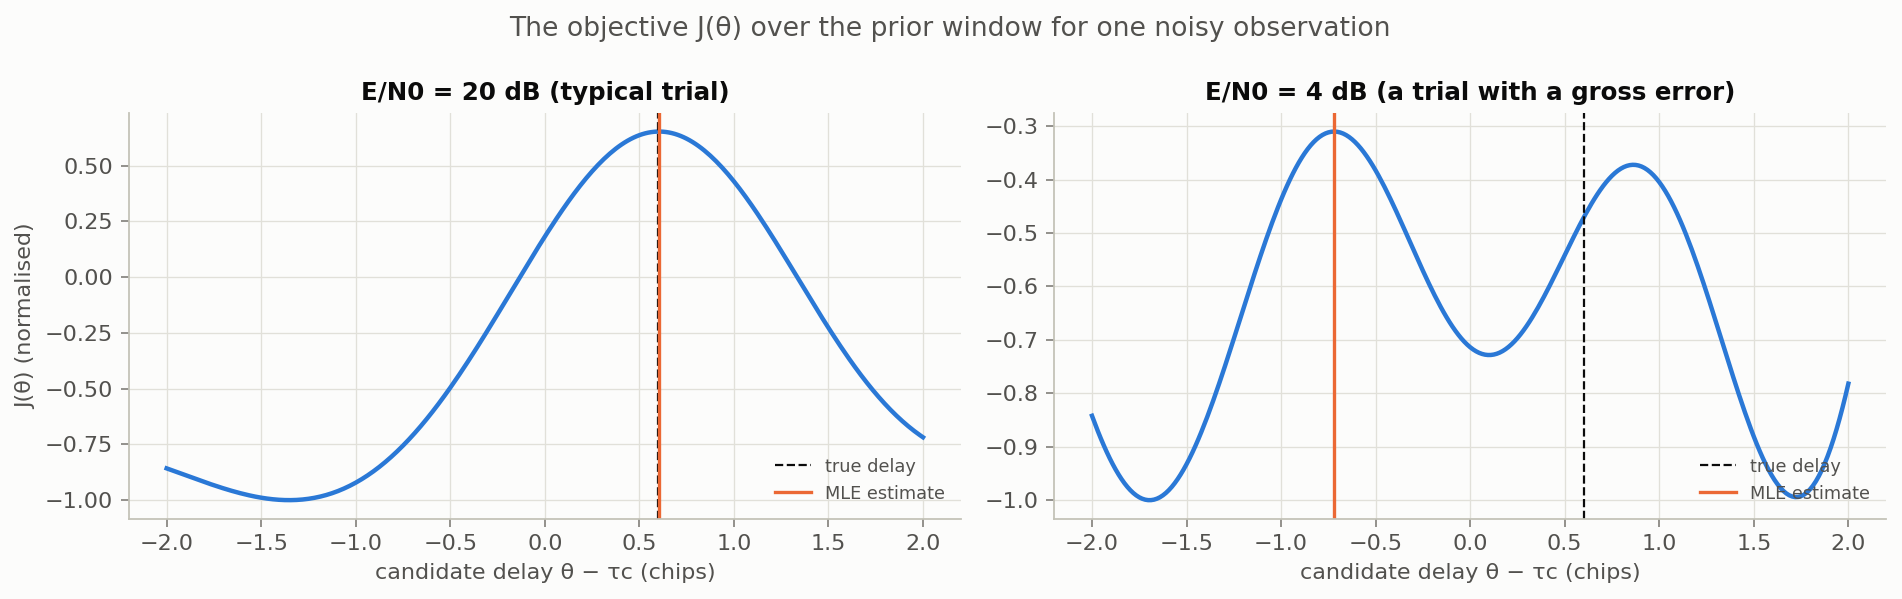
\includegraphics[width=\textwidth]{s1_objective_one_trial.png}
\caption{The MLE objective over the search window for one observation. Left (20\,dB): one clear peak at the true delay.
Right (4\,dB, a trial selected to show the mechanism): a noise-induced bump 1.3 chips away is higher than the true peak,
so the estimator jumps there.}
\end{figure}

% =====================================================================
\section{Mathematical toolkit (with proofs)}\label{sec:toolkit}
Everything later rests on six facts. Each is proved here so nothing is taken on trust.

\subsection{Bias, variance and mean-squared error}\label{sec:bias}
For an estimator $\hat\tau$ with error $e=\hat\tau-\tau$:
\begin{equation}
  \underbrace{\E[e^2]}_{\text{MSE}} = \underbrace{\var(\hat\tau)}_{\text{spread}} + \underbrace{\big(\E[\hat\tau]-\tau\big)^2}_{\text{bias}^2}.
\end{equation}
\begin{proofbox}
Write $e=(\hat\tau-\E\hat\tau)+(\E\hat\tau-\tau)$, square and take expectations; the cross term is
$2(\E\hat\tau-\tau)\,\E[\hat\tau-\E\hat\tau]=0$. \hfill$\blacksquare$
\end{proofbox}
\begin{whybox}
Below threshold our estimators become \textbf{biased} (a delay near the edge of the window is pulled inward). The CRLB
bounds only the variance of \emph{unbiased} estimators, while the ZZB bounds the MSE. So all our plots use MSE.
\end{whybox}

\subsection{The Gaussian likelihood}
If $r[n]=\mu_n(\theta)+w[n]$ with $w[n]\sim\mathcal N(0,\sigma^2)$ independent,
\begin{equation}
p(\br;\theta)=\prod_n\frac{1}{\sqrt{2\pi\sigma^2}}\exp\!\Big(-\frac{(r[n]-\mu_n(\theta))^2}{2\sigma^2}\Big),\qquad
\ln p(\br;\theta)=\text{const}-\frac{1}{2\sigma^2}\sum_n\big(r[n]-\mu_n(\theta)\big)^2 .
\end{equation}
Maximising the likelihood is the same as \textbf{minimising the squared distance} between data and model (least squares).

\subsection{The Q-function and binary detection in Gaussian noise}\label{sec:detection}
$Q(x)=\int_x^\infty \frac{1}{\sqrt{2\pi}}e^{-u^2/2}\,du=P(Z>x)$ for $Z\sim\mathcal N(0,1)$; $Q(0)=\tfrac12$, $Q$ decreases,
$Q(x)\le\tfrac12e^{-x^2/2}$ for $x\ge0$.
\begin{resultbox}[Result: minimum error probability between two known signals]
Observe $\br=\bs_i+\bw$, $i\in\{0,1\}$, equally likely, $\bw\sim\mathcal N(0,\sigma^2 I)$. The smallest possible
probability of deciding wrongly is
\begin{equation}
  P_{\min}=Q\!\left(\frac{\|\bs_1-\bs_0\|}{2\sigma}\right).
\end{equation}
\end{resultbox}
\begin{proofbox}
With equal priors the optimal (MAP) rule picks the signal closer to $\br$: decide 1 iff
$\|\br-\bs_1\|^2<\|\br-\bs_0\|^2$, i.e.\ $T=\langle\br,\bs_1-\bs_0\rangle>\tfrac12(\|\bs_1\|^2-\|\bs_0\|^2)$.
Under hypothesis 0, $T$ is Gaussian with mean $\langle\bs_0,\bs_1-\bs_0\rangle$ and standard deviation
$\sigma\|\bs_1-\bs_0\|$. The distance from this mean to the threshold is $\tfrac12\|\bs_1-\bs_0\|^2$, so the error probability
under 0 is $Q\big(\tfrac12\|\bs_1-\bs_0\|^2/(\sigma\|\bs_1-\bs_0\|)\big)=Q(\|\bs_1-\bs_0\|/2\sigma)$, and by symmetry the same
under 1.\hfill$\blacksquare$
\end{proofbox}

\subsection{Fisher information and the Cramér--Rao inequality}\label{sec:crlbthm}
The \textbf{score} is $S(\theta)=\partial_\theta\ln p(\br;\theta)$; the \textbf{Fisher information} is $I(\theta)=\E[S(\theta)^2]$.
\begin{resultbox}[Theorem (CRLB)]
If $\E[S(\theta)]=0$ (regularity) and $\hat\theta$ is unbiased, then $\var(\hat\theta)\ge 1/I(\theta)$.
\end{resultbox}
\begin{proofbox}
Unbiasedness: $\int\hat\theta(\br)\,p(\br;\theta)\,d\br=\theta$. Differentiating, $\E[\hat\theta S]=1$; since $\E[S]=0$,
also $\E[(\hat\theta-\theta)S]=1$. By Cauchy--Schwarz,
$1=\E[(\hat\theta-\theta)S]^2\le\E[(\hat\theta-\theta)^2]\,\E[S^2]=\var(\hat\theta)\,I(\theta)$.\hfill$\blacksquare$

Equality needs $S\propto\hat\theta-\theta$; then the estimator is \emph{efficient}. The MLE becomes efficient as the SNR grows.
\end{proofbox}

\subsection{Autocorrelation, bandwidth and Parseval}\label{sec:parseval}
The normalised autocorrelation is $\rho(h)=\sum_n s(t_n)s(t_n-h)\big/\sum_n s(t_n)^2$ with $\rho(0)=1$, $|\rho(h)|\le1$.
The \textbf{mean-square (Gabor) bandwidth} is
\begin{equation}
  \beta^2=\frac{\sum_n s'(t_n)^2}{\sum_n s(t_n)^2}=\frac{\int(2\pi f)^2|S(f)|^2\,df}{\int|S(f)|^2\,df},
\end{equation}
the second form by Parseval, since the spectrum of $s'$ is $j2\pi f\,S(f)$.
\begin{proofbox}[Fact: $\rho''(0)=-\beta^2$]
$\frac{d^2}{dh^2}\sum_n s(t_n)s(t_n-h)\big|_{h=0}=\sum_n s(t_n)s''(t_n)$. Summation by parts (exact for a band-limited signal
sampled above Nyquist) gives $\sum s\,s''=-\sum s'^2$; dividing by $\sum s^2$, $\rho''(0)=-\beta^2$, hence
$1-\rho(h)\approx\tfrac12\beta^2h^2$ for small $h$.\hfill$\blacksquare$
\end{proofbox}
\begin{warnbox}[A subtlety we hit]
Summation by parts needs a continuous slope. A hard-truncated pulse left a tiny slope jump; samples landing on it made the
measured curvature disagree with $\beta^2$. We fixed it by tapering the pulse smoothly over its last chip
(Section~\ref{sec:decisions}).
\end{warnbox}

\subsection{A tail-integral identity}\label{sec:tail}
For a non-negative random variable $X$: $\;\E[X^2]=\int_0^\infty 2x\,P(X\ge x)\,dx.$
\begin{proofbox}
$X^2=\int_0^X2x\,dx=\int_0^\infty 2x\,\mathbf 1\{X\ge x\}\,dx$; take expectations and swap (Tonelli, non-negative integrand).\hfill$\blacksquare$
\end{proofbox}
This identity is the first step of the Ziv--Zakai bound: it turns the MSE into a sum over error \emph{sizes}.

% =====================================================================
\section{The signal model and why each choice was made}\label{sec:model}
\textit{Notebook 00. Every estimator and bound uses exactly this model.}

\subsection{The model}
\begin{equation}
  s(t)=\sum_{k=0}^{N_c-1}a_k\,p(t-k),\qquad r[n]=s(t_n-\tau)+w[n],\quad t_n=\tfrac n4,\quad w[n]\sim\mathcal N(0,\sigma^2),
\end{equation}
with a known pilot $a_k\in\{\pm1\}$ of $N_c=64$ chips, time in chips ($T_c=1$), and the raised-cosine pulse
\begin{equation}
  p(t)=\operatorname{sinc}(t)\,\frac{\cos(\pi\alpha t)}{1-(2\alpha t)^2},\qquad \alpha=0.5,
\end{equation}
smoothly truncated to $|t|\le6$ chips. $p$ is a \textbf{Nyquist pulse}: $p(0)=1$, $p(k)=0$ at every other integer. The delay
has a uniform prior $\tau\sim\mathcal U[\tau_c-T_a/2,\tau_c+T_a/2]$ with $T_a=4$ chips.

\begin{figure}[h]
\centering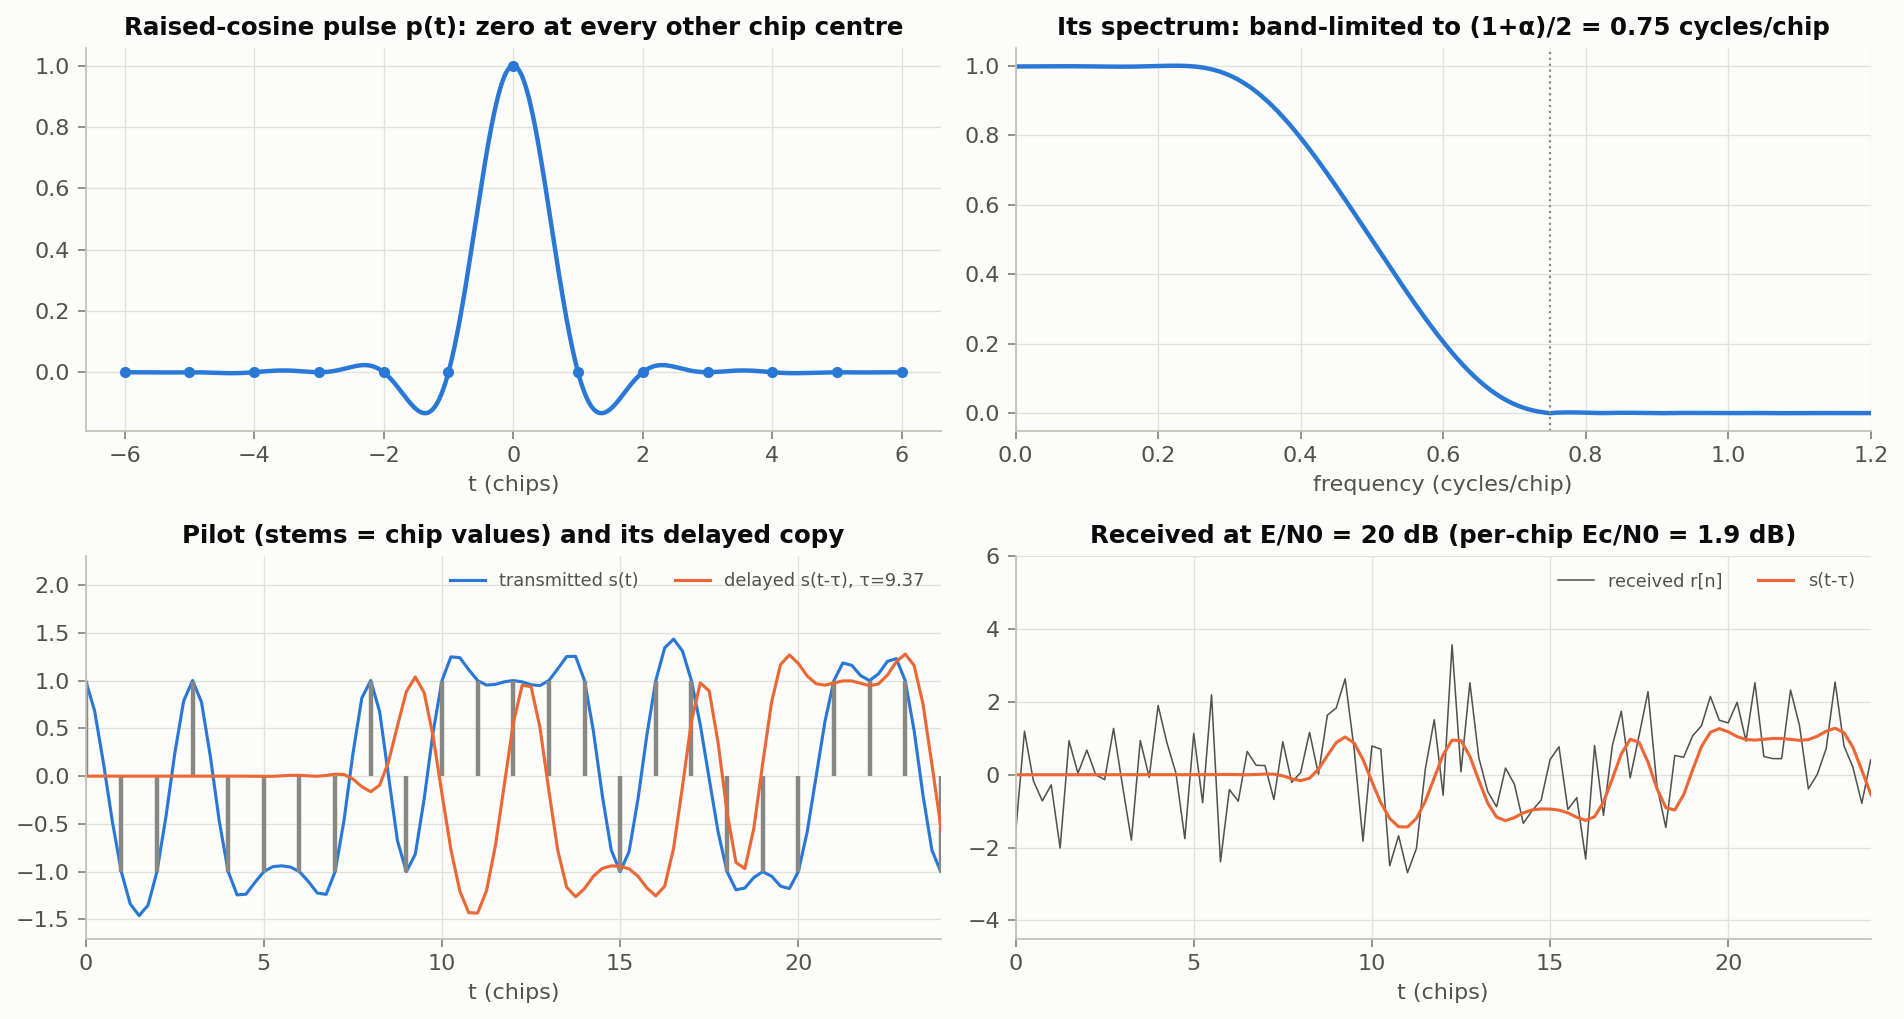
\includegraphics[width=\textwidth]{s0_signal_model.png}
\caption{The pulse and its spectrum (band-limited to 0.75 cycles/chip), the pilot with its delayed copy, and what the
receiver sees at $\ENo=20$\,dB.}
\end{figure}

\subsection{The SNR --- derivation}
White noise has two-sided spectral density $N_0/2$; sampling at rate $f_s$ after an ideal band-limit gives sample
variance $\sigma^2=\tfrac{N_0}{2}f_s$. The signal energy is $E=\int s^2dt=T_s\sum_n s[n]^2$. Therefore
\begin{equation}
  \frac{E}{N_0}=\frac{T_s\sum_n s[n]^2}{2\sigma^2T_s}=\frac{\sum_n s[n]^2}{2\sigma^2}\quad\Longrightarrow\quad
  \sigma^2=\frac{\sum_n s[n]^2}{2\,\ENo}.
\end{equation}
All plots use the \textbf{total batch} $\ENo$; per chip, $E_c/N_0=\ENo-10\log_{10}64=\ENo-18.1$\,dB. Check: requesting 10
gives a measured 10.03.

\subsection{Decisions and their reasons}
\begin{center}
\begin{tabularx}{\textwidth}{>{\raggedright\arraybackslash}p{3.6cm}>{\raggedright\arraybackslash}X>{\raggedright\arraybackslash}X}
\toprule
\textbf{Decision} & \textbf{Reason} & \textbf{What goes wrong otherwise}\\
\midrule
Raised-cosine pulse & band-limited like a real receiver; analytic spectrum & rectangular chips: $\beta^2=\infty$, CRLB $=0$\\
4 samples per chip & spectrum ends at 0.75 cycles/chip $<$ Nyquist (2) & aliasing; sums $\neq$ integrals\\
Analytic delay & $s(t_n-\tau)$ evaluated exactly & interpolation error at high SNR\\
Known pilot, coherent, AWGN & closed-form likelihood, CRLB and ZZB & nuisance parameters (future work)\\
Uniform prior, $T_a=4$ & the ZZB is Bayesian and needs a prior & $T_a=1$ masks the threshold\\
SNR = batch $\ENo$ & both bounds depend on total energy & per-sample SNR hides pilot length\\
MSE as metric & estimators biased below threshold; ZZB bounds MSE & variance hides the bias\\
\bottomrule
\end{tabularx}
\end{center}
\begin{whybox}[Why the model changed after the first Sprint-1 script]
The original script (archived) used a 127-chip m-sequence, a Gaussian filter, a fixed delay and per-sample SNR, and showed
the same qualitative result. It was replaced because the ZZB needs a \emph{random} delay with a prior, the bounds are naturally
written in $\ENo$, and the raised cosine makes the CRLB checkable analytically.
\end{whybox}
\begin{figure}[h]
\centering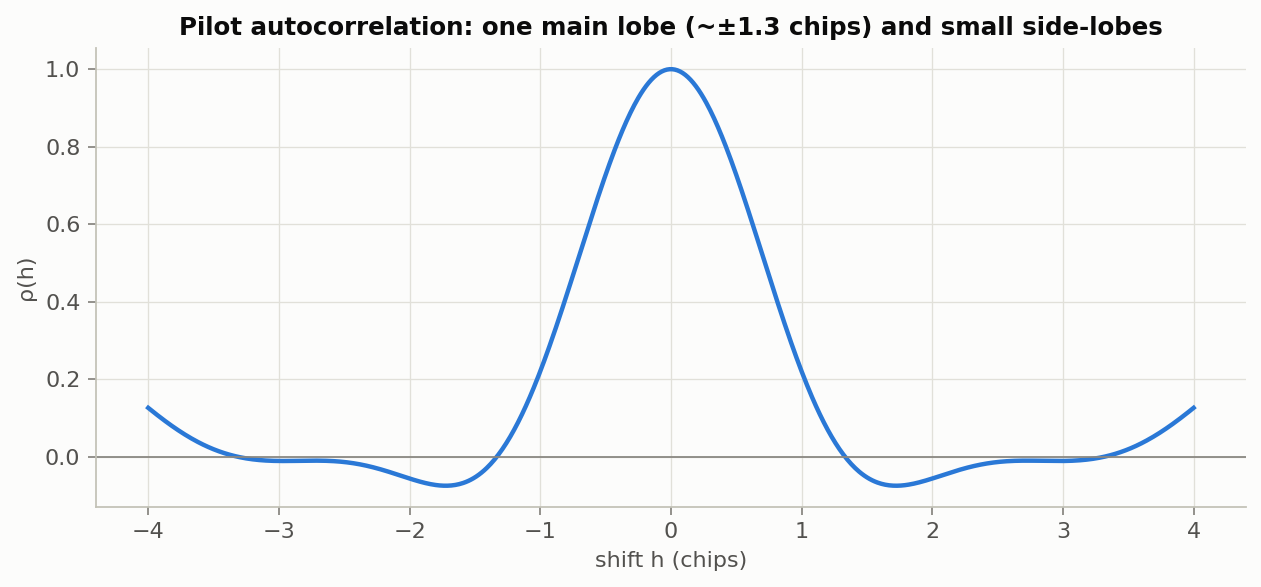
\includegraphics[width=0.8\textwidth]{s0_autocorrelation.png}
\caption{The pilot's autocorrelation: main lobe to about $\pm1.34$ chips, side-lobes at most 0.13 beyond 1.5 chips. Its
curvature at $h=0$ sets the CRLB; its side-lobes and the prior width set the ZZB.}
\end{figure}

% =====================================================================
\part{Estimators and bounds}
\section{Sprint 1 --- the batch maximum-likelihood estimator}\label{sec:mle}
\textit{Notebook 01.} \done

\subsection{Derivation: the MLE is a correlator}
With $\mu_n(\theta)=s(t_n-\theta)$ the Gaussian log-likelihood expands as
\begin{equation}
\ln p(\br;\theta)=\text{const}-\frac{1}{2\sigma^2}\sum_n r[n]^2+\frac{1}{\sigma^2}\Big(\sum_n r[n]\,s(t_n-\theta)-\tfrac12\sum_n s(t_n-\theta)^2\Big).
\end{equation}
The first sum does not depend on $\theta$, hence
\begin{resultbox}
\begin{equation}
\hat\tau_{\rm ML}=\arg\max_{\theta\in\text{window}}J(\theta),\qquad
J(\theta)=\underbrace{\sum_n r[n]\,s(t_n-\theta)}_{\text{correlation with a shifted replica}}-\tfrac12\underbrace{\sum_n s(t_n-\theta)^2}_{\text{replica energy}}.
\end{equation}
\end{resultbox}
\begin{itemize}
\item \textbf{Interpretation:} slide a clean replica over the data and pick the best match --- a matched filter.
\item \textbf{No SNR needed:} $\sigma^2$ scales the whole function, so it does not move the arg-max.
\item \textbf{Energy term:} almost constant (the pulse train stays inside the window); kept so the estimator is exactly the MLE.
\item \textbf{Window constraint:} with a uniform prior, the MAP estimator equals this constrained MLE.
\end{itemize}

\subsection{Sub-grid refinement --- derivation}
$J$ is computed on a grid of step $\Delta=1/64$ chip. Fit $J(\theta_g+x\Delta)\approx ax^2+bx+c$ through the best grid point
and its neighbours: $J_{g\pm1}=a\pm b+c$, $J_g=c$, so $a=\tfrac12(J_{g-1}-2J_g+J_{g+1})$, $b=\tfrac12(J_{g+1}-J_{g-1})$. The vertex
$x^\star=-b/2a$ gives
\begin{equation}
\hat\theta=\theta_g+\frac{\Delta}{2}\,\frac{J_{g-1}-J_{g+1}}{J_{g-1}-2J_g+J_{g+1}}.
\end{equation}
Without noise the error is 0.02\% of the CRLB at 30\,dB --- negligible.

\subsection{The MMSE estimator (posterior mean)}
With the uniform prior, $p(\theta\mid\br)\propto\exp(J(\theta)/\sigma^2)$ on the window, and the MSE-optimal estimator is
\begin{equation}
\hat\tau_{\rm MMSE}=\frac{\int\theta\,e^{J(\theta)/\sigma^2}d\theta}{\int e^{J(\theta)/\sigma^2}d\theta}.
\end{equation}
\begin{proofbox}[Why the posterior mean minimises MSE]
For any $g(\br)$, $\E[(\tau-g)^2\mid\br]=\var(\tau\mid\br)+(\E[\tau\mid\br]-g)^2$, minimised by $g=\E[\tau\mid\br]$; averaging over
$\br$ keeps the minimum.\hfill$\blacksquare$
\end{proofbox}
It is computed from the same grid of $J$ values but needs $\sigma^2$. It matters because the ZZB bounds \emph{every}
estimator, so the fair comparison for the bound is the best one (Section~\ref{sec:res6}). It is an extension beyond the brief.

% =====================================================================
\section{Sprint 3 --- the Cramér--Rao lower bound for our model}\label{sec:crlb}
\textit{Notebook 03.} \done

\subsection{Derivation in four steps}
\begin{enumerate}
\item \textbf{Score:} $\partial_\tau\ln p=\frac1{\sigma^2}\sum_n(r[n]-\mu_n)\mu_n'=\frac1{\sigma^2}\sum_n w[n]\,\mu_n'(\tau)$; its mean is 0 (regularity holds).
\item \textbf{Fisher information:} $I=\E[(\partial_\tau\ln p)^2]=\frac{1}{\sigma^4}\sum_n\sum_m\E[w_nw_m]\mu_n'\mu_m'=\frac1{\sigma^2}\sum_n\mu_n'^2$.
\item \textbf{Delay model:} $\mu_n'(\tau)=\partial_\tau s(t_n-\tau)=-s'(t_n-\tau)$, so $I=\frac1{\sigma^2}\sum_n s'(t_n-\tau)^2$.
\item \textbf{Physical form:} substitute $\sigma^2=\sum s^2/(2\ENo)$:
\end{enumerate}
\begin{resultbox}
\begin{equation}
\var(\hat\tau)\ \ge\ \text{CRLB}=\frac{1}{2\,(\ENo)\,\beta^2}=\frac{1}{2\,N_c\,(E_c/N_0)\,\beta^2}.
\end{equation}
\end{resultbox}
\begin{itemize}
\item \textbf{Energy:} doubling the pilot length or the SNR halves the CRLB.
\item \textbf{Bandwidth:} steeper edges (larger $\beta^2$) give a sharper peak; rectangular chips give $\beta^2=\infty$.
\item \textbf{Independent of $\tau$} while the pulse train stays inside the window ($\beta^2$ varies by $10^{-5}$ across delays).
\end{itemize}

\subsection{Checks}
$\beta^2$ from the spectrum (FFT at 64 samples/chip) is 2.4470; from the samples (the code) 2.4481 --- agreement to 0.05\%.
For the isolated pulse $\beta^2=2.838$; averaged over 400 random pilots, 2.873.

\subsection{A finding: the CRLB depends on the pilot}
Over 400 random 64-chip pilots $\beta^2$ ranges from 1.77 to 4.27 --- a factor 2.4 in the CRLB. Every estimator and bound must
therefore use the \emph{same} pilot, and thresholds defined relative to the CRLB move from pilot to pilot.
\begin{figure}[h]
\centering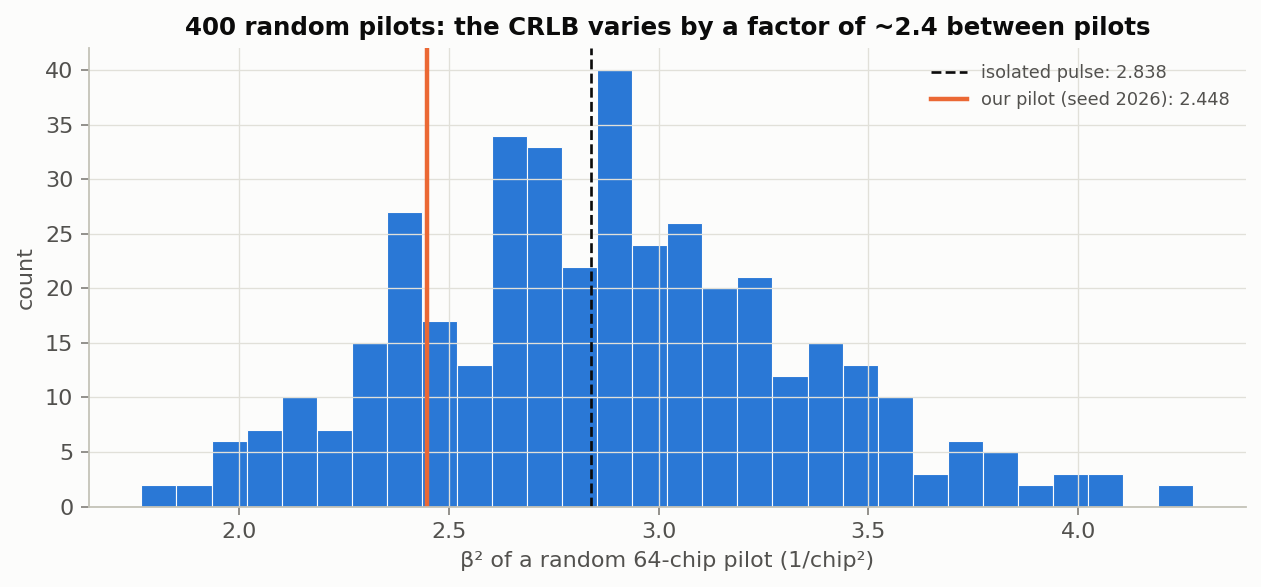
\includegraphics[width=0.72\textwidth]{s3_beta2_pilots.png}
\caption{$\beta^2$ for 400 random pilots; our pilot (seed 2026) has 2.448.}
\end{figure}

\subsection{Where the CRLB stops making sense --- three reasons}
\begin{enumerate}
\item \textbf{It assumes unbiasedness.} For a delay 0.5 chip from the edge the MLE's bias is $-1.18$ chips at $-10$\,dB and
$-0.47$ chips at 2\,dB (pulled towards the centre), $\approx0$ above 14\,dB.
\item \textbf{It is local.} $I(\tau)$ involves only $s'$ at the true delay --- the curvature of the true peak.
\item \textbf{It ignores the prior.} Below about $-8$\,dB the CRLB exceeds the prior variance $T_a^2/12$.
\end{enumerate}
\textbf{Edge effect (small).} Within 0.05 chip of a window edge the constrained MLE reaches MSE/CRLB $=0.63$ at 20\,dB; this
changes the averaged MSE by about 1\%.
\begin{figure}[h]
\centering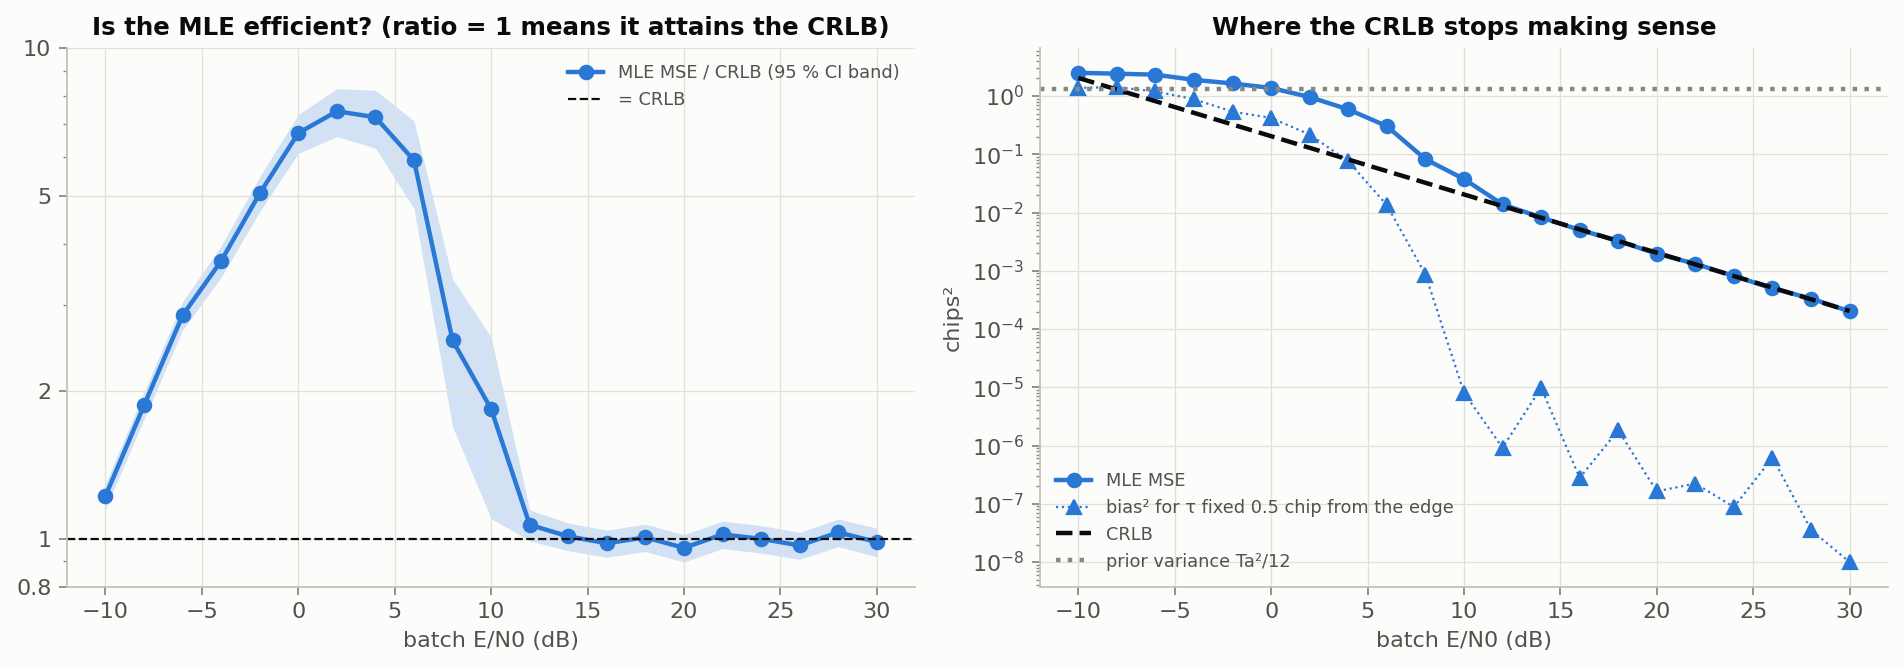
\includegraphics[width=\textwidth]{s3_crlb_vs_mle.png}
\caption{Left: MLE MSE/CRLB with 95\% band --- equal to 1 above $\approx$12--14\,dB. Right: MSE, CRLB, prior variance and the
conditional bias$^2$ for a delay near the edge.}
\end{figure}

% =====================================================================
\section{The threshold effect}\label{sec:threshold}
Above threshold the estimate lands on the true correlation peak and errors are small and Gaussian. In the threshold region
a fraction $P$ of trials are \textbf{gross errors} ($|e|>0.5$ chip, outside the main lobe). The idea behind the method of
interval errors (MIE):
\begin{equation}
\text{MSE}\approx(1-P)\cdot\text{CRLB}+P\cdot\sigma^2_{\rm gross},
\end{equation}
with $\sigma^2_{\rm gross}$ of order the prior width squared. Since $\sigma^2_{\rm gross}\gg$ CRLB, even $P=1\%$ dominates: at
10\,dB a 1\% rate of 2-chip errors adds 0.04\,chips$^2$, twice the CRLB. The threshold is a change in the \textbf{type} of
error, not a gradual widening.
\begin{figure}[h]
\centering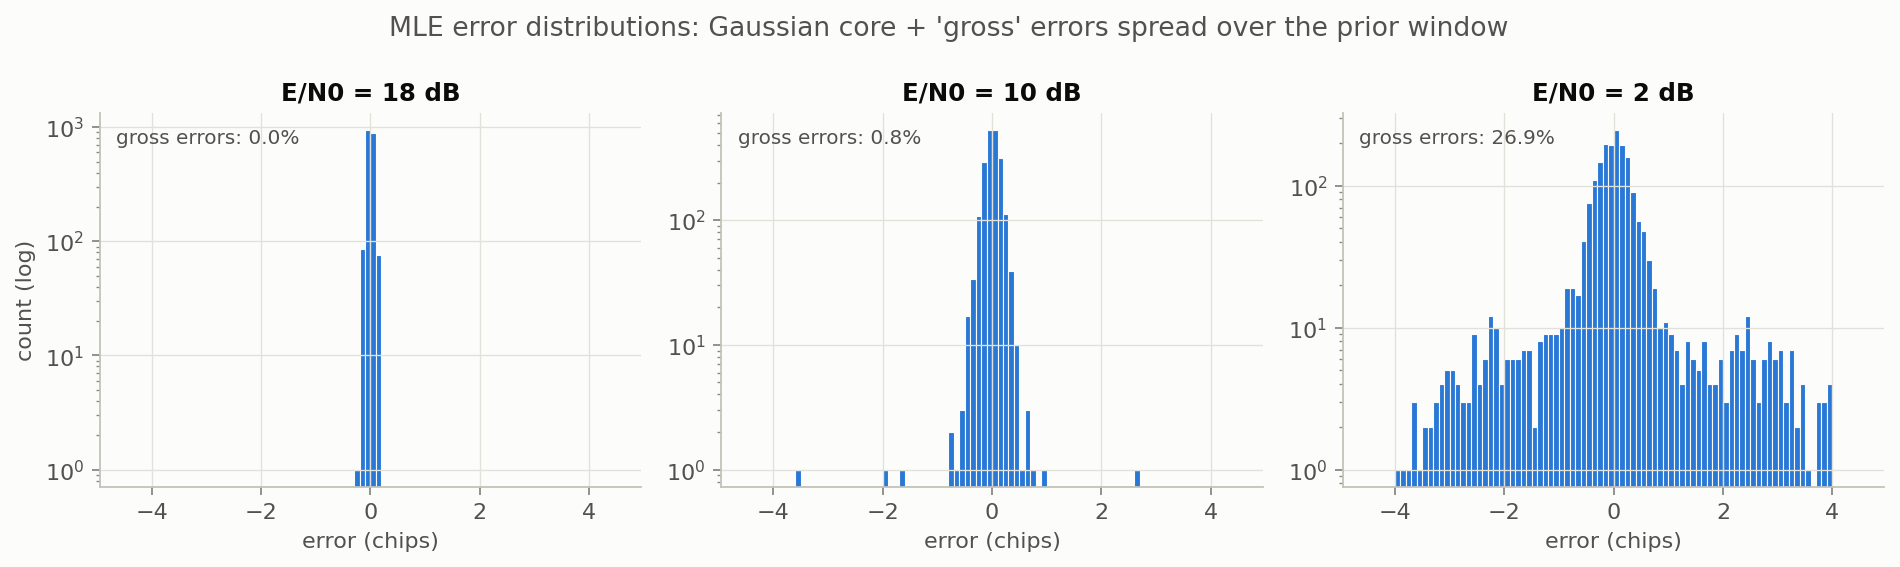
\includegraphics[width=\textwidth]{s1_mle_error_hist.png}
\caption{MLE error histograms (log count) at 18, 10 and 2\,dB: a narrow Gaussian core, then a growing population of gross
errors spread over the window.}
\end{figure}
\textbf{Very low SNR.} On pure noise the MLE's MSE is 3.09\,chips$^2$ --- above the prior variance 1.33 --- because the arg-max
of a noise process piles up at the window edges (about 20\% of estimates sit exactly on an edge). The MMSE estimator tends to
the window centre and its MSE to $T_a^2/12$.

% =====================================================================
\section{Sprint 4 --- the Ziv--Zakai bound, derived for this problem}\label{sec:zzb}
\textit{Notebook 04.} \done\ (derivation; numerical evaluation also done, Sprint-5 material)

\subsection{The idea}
If an estimator could locate $\tau$ to within $h/2$, it could tell ``$\tau=\varphi$'' from ``$\tau=\varphi+h$''. Detection
theory gives the best possible error rate for that test, so the estimator must make errors of size about $h/2$ at least that
often. Doing this for \textbf{every} separation $h$ gives a lower bound on the MSE that sees both local and distant errors.

\subsection{Derivation, step by step}
\textbf{Step 1 --- MSE as a sum over error sizes.} Apply Section~\ref{sec:tail} to $X=|e|$ and substitute $x=h/2$:
\begin{equation}\label{eq:z1}
\text{MSE}=\int_0^\infty\frac h2\,P\!\left(|e|\ge\tfrac h2\right)dh.
\end{equation}
\textbf{Step 2 --- split by direction and shift.} Condition on the true delay; substitute $\varphi\to\varphi+h$ in the second part:
\begin{equation}\label{eq:z2}
P(|e|\ge\tfrac h2)=\int\Big[p(\varphi)P(e\ge\tfrac h2\mid\varphi)+p(\varphi+h)P(e\le-\tfrac h2\mid\varphi+h)\Big]d\varphi.
\end{equation}
\textbf{Step 3 --- recognise a detector.} Fix $\varphi,h$; consider $H_0:\tau=\varphi$ vs $H_1:\tau=\varphi+h$ with weights
$p(\varphi)$, $p(\varphi+h)$. Decide $H_1$ iff $\hat\tau\ge\varphi+h/2$. Under $H_0$ it errs exactly when $e\ge h/2$; under $H_1$
exactly when $e<-h/2$. So the bracket in \eqref{eq:z2} is $(p(\varphi)+p(\varphi+h))\times$ this detector's error
probability, which is at least the optimal one:
\begin{equation}\label{eq:z3}
P(|e|\ge\tfrac h2)\ \ge\ \int\big(p(\varphi)+p(\varphi+h)\big)\,P_{\min}(\varphi,\varphi+h)\,d\varphi.
\end{equation}
\textbf{Step 4 --- combine and valley-fill.} Substituting \eqref{eq:z3} into \eqref{eq:z1}:
\begin{equation}
\text{MSE}\ \ge\ \frac12\int_0^\infty h\;\VF\Big\{\int\big(p(\varphi)+p(\varphi+h)\big)P_{\min}\,d\varphi\Big\}\,dh,\qquad
\VF\{g\}(h)=\max_{\eta\ge0}g(h+\eta).
\end{equation}
Valley filling is allowed because the left side of \eqref{eq:z3} decreases in $h$ (Bell et al., 1997). For our pilot it
changes the bound by less than 0.01\%.

\textbf{Step 5 --- the optimal detector for our signals.} The two hypotheses are known signals in white Gaussian noise,
equally likely under the uniform prior. By Section~\ref{sec:detection}, $P_{\min}=Q(\|\bs_1-\bs_0\|/2\sigma)$ and
$\|\bs_1-\bs_0\|^2=2\sum s^2(1-\rho(h))$. With $\sum s^2/(2\sigma^2)=\ENo$:
\begin{equation}
P_{\min}(h)=Q\!\left(\sqrt{\tfrac{E}{N_0}\big(1-\rho(h)\big)}\right).
\end{equation}
Two delays are hard to distinguish when the signal is weak \emph{or} when the shifted signals look alike. $P_{\min}$ does not
depend on $\varphi$ (verified to $2\cdot10^{-5}$).

\textbf{Step 6 --- the uniform prior.} Both $\varphi$ and $\varphi+h$ must lie in the window (a range of length $T_a-h$, density
$1/T_a$), so $\int(p(\varphi)+p(\varphi+h))d\varphi=2(1-h/T_a)$ for $0\le h\le T_a$. The factors $\frac12$ and 2 cancel:
\begin{resultbox}[Result --- the ZZB for our problem]
\begin{equation}
\text{ZZB}=\int_0^{T_a}h\;\VF\Big\{\Big(1-\frac h{T_a}\Big)\,Q\Big(\sqrt{\tfrac{E}{N_0}\,(1-\rho(h))}\Big)\Big\}\,dh.
\end{equation}
\end{resultbox}

\subsection{The two limits --- proofs}
\begin{proofbox}[No signal: ZZB $\to T_a^2/12$]
$\ENo\to0$ gives $Q(0)=\frac12$: $\int_0^{T_a}\frac h2(1-\frac h{T_a})dh=\frac{T_a^2}{4}-\frac{T_a^2}{6}=\frac{T_a^2}{12}$, the prior
variance. No estimator can do better without data; the window centre achieves it.\hfill$\blacksquare$
\end{proofbox}
\begin{proofbox}[Strong signal: ZZB $\to$ CRLB]
Only small $h$ contribute; there $1-\rho\approx\frac12\beta^2h^2$ and $1-h/T_a\approx1$. With $a^2=\frac12(\ENo)\beta^2$, using
$Q'(x)=-\phi(x)$ and integrating by parts,
\begin{equation*}
\int_0^\infty hQ(ah)\,dh=\Big[\tfrac{h^2}{2}Q(ah)\Big]_0^\infty+\frac a2\int_0^\infty h^2\phi(ah)\,dh=\frac{1}{2a^2}\int_0^\infty u^2\phi(u)\,du=\frac{1}{4a^2},
\end{equation*}
and $1/(4a^2)=1/(2(\ENo)\beta^2)=$ CRLB.\hfill$\blacksquare$
\end{proofbox}
Numerically: 1.3323 at zero SNR ($T_a^2/12=1.3333$) and ZZB/CRLB $=0.997$ at 40\,dB.

\subsection{Intuition and how to explain it}
\begin{figure}[h]
\centering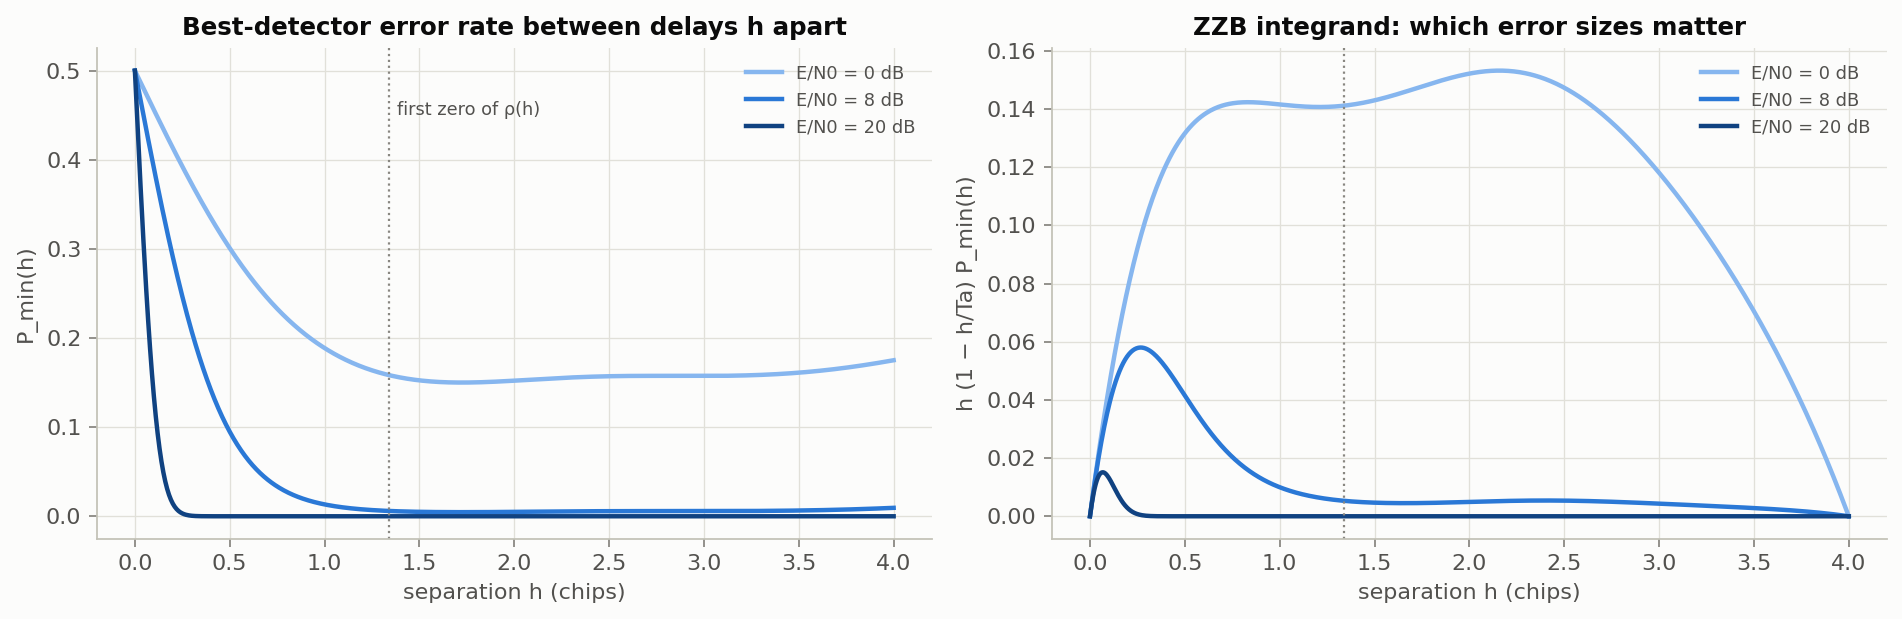
\includegraphics[width=\textwidth]{s4_zzb_intuition.png}
\caption{Left: $P_{\min}(h)$ at 0, 8, 20\,dB. Right: the integrand $h(1-h/T_a)P_{\min}(h)$ --- at 20\,dB only tiny separations
contribute (CRLB-like); at 0\,dB distant separations contribute heavily.}
\end{figure}
\begin{saybox}
``If an estimator is usually within half a chip, I can use it to tell delay $\varphi$ from $\varphi$ plus one chip. Detection
theory says how often \emph{any} detector must confuse those two --- that depends on the SNR and on how similar the shifted
signals are. So the estimator must make errors that big at least that often. Summing over every separation gives a lower
bound on the MSE. At high SNR only tiny separations are confused and I recover the CRLB; at low SNR distant delays are
confused and the bound rises --- the threshold. With no signal, the bound is the prior variance.''
\end{saybox}
\begin{figure}[h]
\centering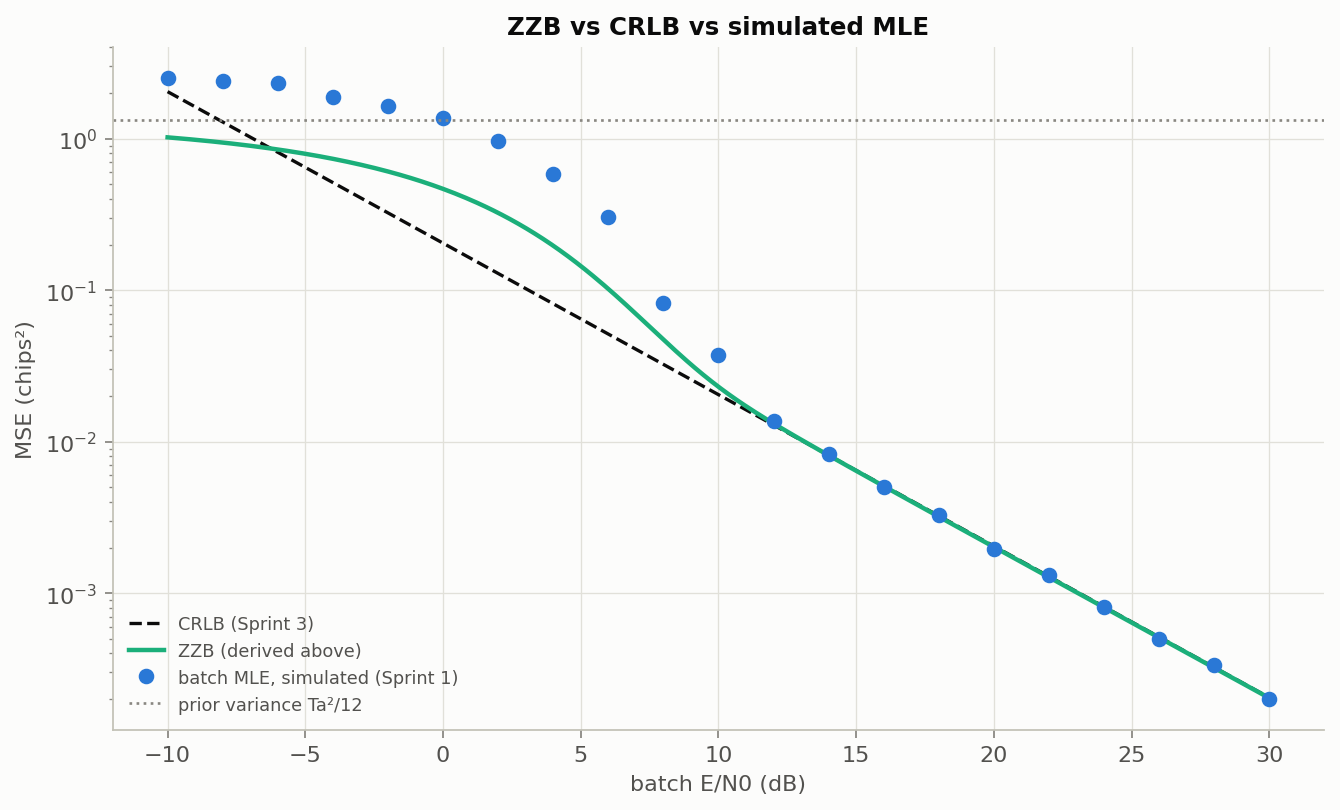
\includegraphics[width=0.78\textwidth]{s4_zzb_vs_crlb_vs_mle.png}
\caption{The ZZB reproduces both limits, departs from the CRLB at $\approx6$\,dB, and lies below the simulated MLE everywhere
(within the 95\% Monte Carlo interval).}
\end{figure}

% =====================================================================
\section{Sprint 2 --- the early--late delay-locked loop}\label{sec:dll}
\textit{Notebook 02.} \done

\subsection{The discriminator}
With estimate $\theta$ and error $\varepsilon=\theta-\tau$, correlate with replicas shifted by $\pm d/2$ ($d=0.5$ chip):
\begin{equation}
E=\sum_n r[n]\,s(t_n-\theta+\tfrac d2),\qquad L=\sum_n r[n]\,s(t_n-\theta-\tfrac d2).
\end{equation}
Without noise each is a sample of $R(h)=\sum_n s(t_n)s(t_n-h)$: $E-L=R(\varepsilon-\tfrac d2)-R(\varepsilon+\tfrac d2)$. $R$ is
symmetric with its peak at 0, so $E=L$ at $\varepsilon=0$, and by Taylor expansion
\begin{equation}
E-L\approx-2R'(\tfrac d2)\,\varepsilon=k\,\varepsilon,\qquad k>0.
\end{equation}
The discriminator $D=(E-L)/k\approx\varepsilon$ measures the error; the curve $D(\varepsilon)$ is the \textbf{S-curve}.
\begin{figure}[h]
\centering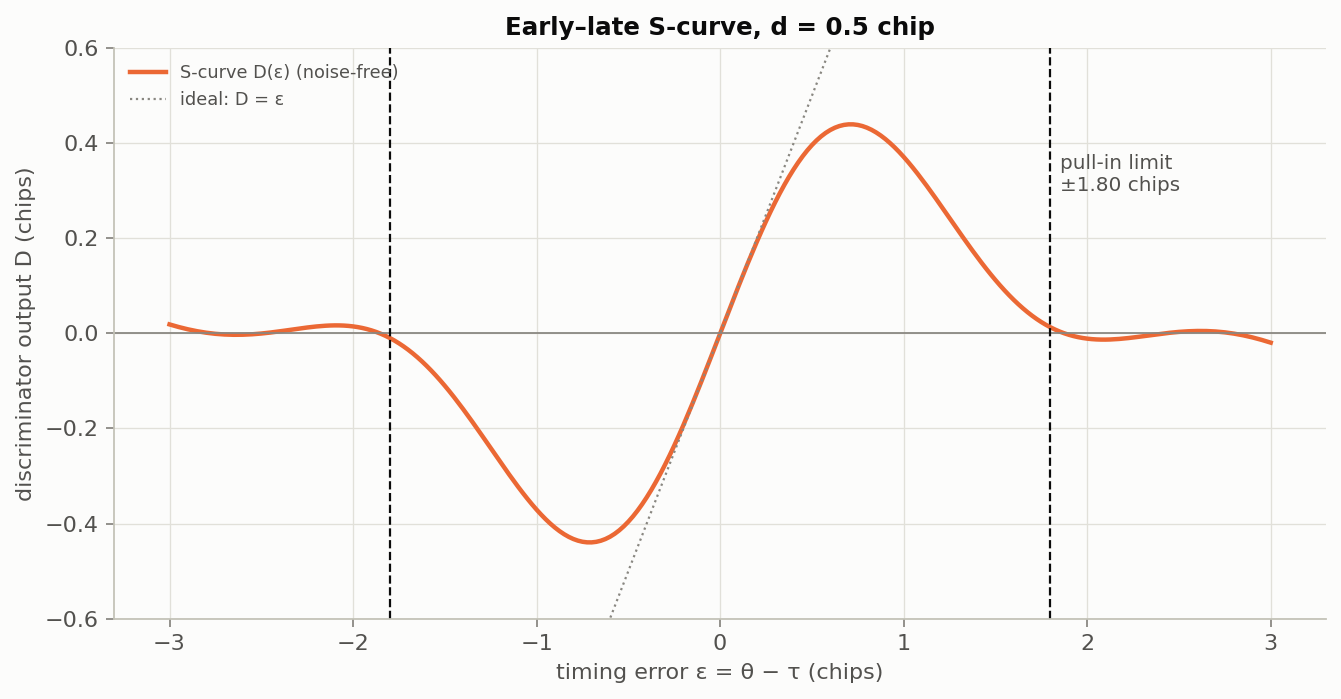
\includegraphics[width=0.75\textwidth]{s2_dll_s_curve.png}
\caption{The S-curve: slope 1 at zero, peak 0.44 at $\varepsilon=0.70$ chip, correct sign out to $\pm1.80$ chips (pull-in range).}
\end{figure}

\subsection{The loop and its noise averaging --- derivation}
Every $M=4$ chips, $\theta_{j+1}=\theta_j-K\,D_j$. In the linear region $D_j=\varepsilon_j+n_j$, so
$\varepsilon_{j+1}=(1-K)\varepsilon_j-Kn_j$.
\begin{itemize}
\item \textbf{Stability:} errors decay iff $|1-K|<1$, i.e.\ $0<K<2$.
\item \textbf{Noise averaging:} impulse response $h_k=K(1-K)^k$; for independent $n_j$ of variance $\sigma_n^2$,
$\var(\varepsilon)=\sigma_n^2\sum_kh_k^2=\sigma_n^2\frac{K^2}{1-(1-K)^2}=\sigma_n^2\frac{K}{2-K}$.
\item Averaging $N$ independent measurements gives $\sigma_n^2/N$, so the loop averages $N_{\rm eff}=(2-K)/K$ updates; its noise
bandwidth is $B_LT_I=\sum h_k^2/(2(\sum h_k)^2)=K/(2(2-K))$.
\end{itemize}
\textbf{Design:} $N_{\rm eff}=64/4=16\Rightarrow K=2/17\approx0.118\Rightarrow1/(2B_L)=64$ chips: the locked loop averages as much
signal as the 64-chip batch. The loop runs 160 updates = 640 chips.

\subsection{Implementation details that were necessary}
\begin{center}
\begin{tabularx}{\textwidth}{>{\raggedright\arraybackslash}p{3.0cm}>{\raggedright\arraybackslash}X>{\raggedright\arraybackslash}X}
\toprule
\textbf{Detail} & \textbf{What we do} & \textbf{What went wrong without it}\\
\midrule
Acquisition & coarse 0.5-chip search over the prior, then track & pull-in is $\pm1.8$ chips; the prior is $\pm2$\\
Block replicas & block $j$'s replica holds only its 4 chips & bias $\approx33\%$ of the CRLB at 30\,dB\\
Offset calibration $b_j$ & subtract each block's noise-free output at zero error & MSE $\approx2\times$ CRLB at 30\,dB; $b_j$ uses only the known pilot\\
Constant gain $\bar k$ & normalise by the average slope & per-block slopes vary 0.29--1.7$\times$; noise blow-up\\
Windows follow $\theta$ & integration windows placed by the loop's own timing & distorted low-SNR behaviour\\
Same pilot, repeated & the 64-chip pilot repeated like a GNSS code & DLL appeared to beat the CRLB\\
\bottomrule
\end{tabularx}
\end{center}

\subsection{Locked accuracy and its theory}
Linearised, $\varepsilon=\langle\bw,G\rangle$ with $G=\sum_jc_jg_j$ ($g_j$ = early-minus-late replica of block $j$,
$c_j=(K/\bar k)\prod_{i>j}(1-Kk_i/\bar k)$), hence exactly $\var(\varepsilon)=\sigma^2\|G\|^2$. Measured DLL MSE/CRLB: 1.088, 1.083,
1.039 ($\pm0.024$) at 15, 20, 25\,dB; theory 1.071.
\begin{warnbox}[Be precise about this number]
``DLL $\approx$ CRLB'' holds \textbf{because we chose $K$}. A narrower loop averages more of its 640 chips and goes \emph{below}
the 64-chip CRLB --- not a violation, since that CRLB does not bound an estimator using 640 chips. The 7\% excess comes from
early--late being a finite-difference approximation of the derivative.
\end{warnbox}
\begin{figure}[h]
\centering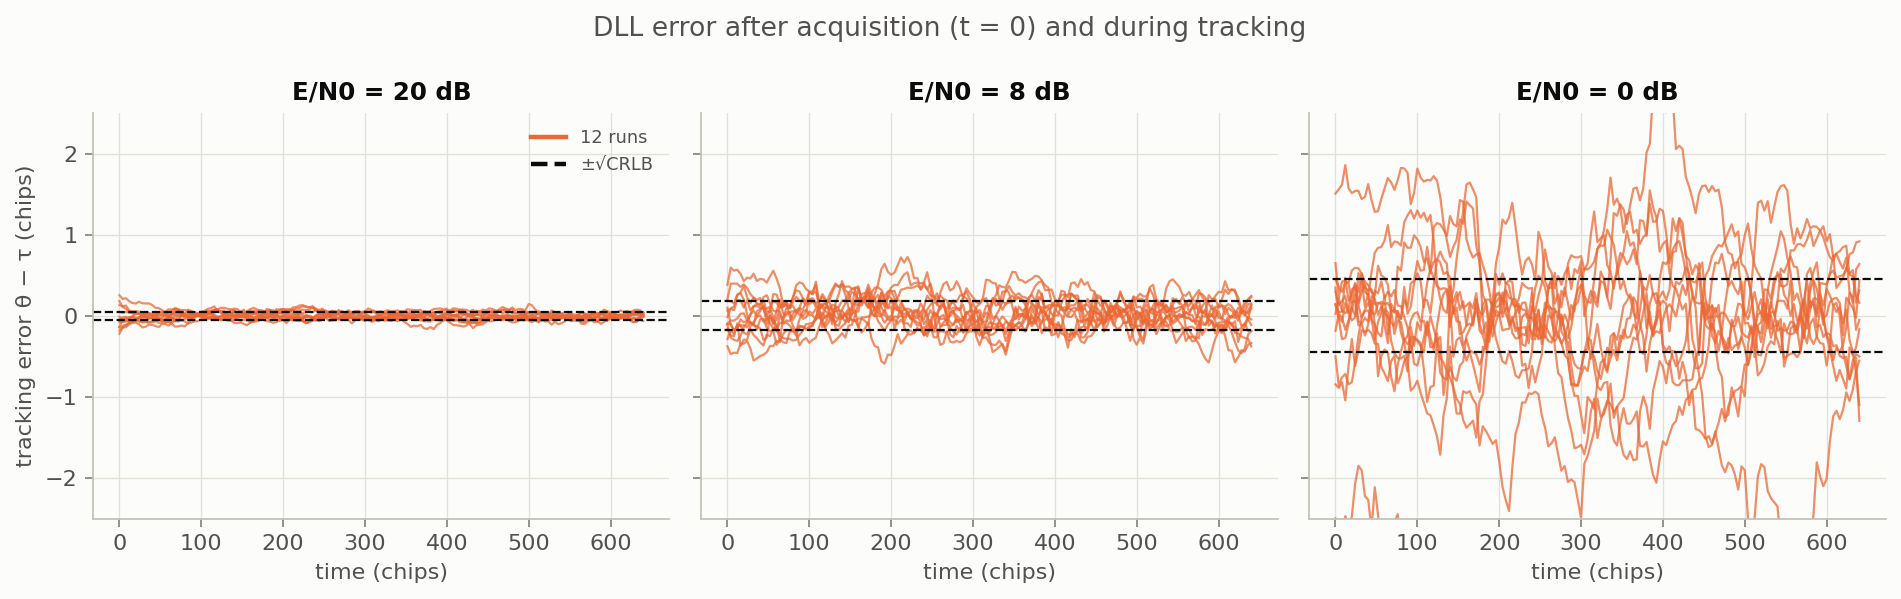
\includegraphics[width=\textwidth]{s2_dll_tracking_run.png}
\caption{DLL error over time, 12 runs at 20, 8 and 0\,dB: tight lock, noisy lock, loss of lock.}
\end{figure}

% =====================================================================
\part{Evidence}
\section{Experimental methodology and validation}\label{sec:method}
\subsection{Monte Carlo}
For each SNR we draw $N$ independent trials (random delay from the prior, fresh noise, one estimate) and report
$\widehat{\text{MSE}}=\frac1N\sum_ie_i^2$, with standard error $\mathrm{sd}(e^2)/\sqrt N$. Near the threshold $e^2$ is heavy-tailed,
so the MSE is uncertain exactly where the threshold is --- hence many trials: 2000 per point (notebooks 01, 05), 20{,}000
(notebook 06, MLE/MMSE), 10{,}000 (notebook 07), 4000 (DLL).

\subsection{Threshold definitions (fixed before looking at results)}
\begin{itemize}
\item \textbf{MSE criterion:} the highest SNR at which MSE/CRLB first exceeds 2 (3\,dB), scanning down from high SNR.
\item \textbf{Gross-error criterion:} the highest SNR at which $P(|e|>0.5\text{ chip})$ first exceeds 1\%. One outlier moves this by
only $1/N$, whereas it can multiply the MSE.
\end{itemize}
Thresholds are interpolated linearly in (dB, $\log y$) between grid points.

\subsection{Confidence intervals by bootstrap}
Resample the $N$ trials at each SNR with replacement, recompute the threshold, repeat 200--300 times, report the 2.5--97.5\%
percentiles. Differences are computed sample by sample from the bootstrap draws; MLE and MMSE share the same noise (paired).

\subsection{How we know the code is right}
\begin{center}
\begin{tabularx}{\textwidth}{>{\raggedright\arraybackslash}X>{\raggedright\arraybackslash}p{6.2cm}}
\toprule
\textbf{Check} & \textbf{Result}\\
\midrule
Analytic checks in every notebook (Nyquist, SNR calibration, noise-free estimators, ZZB limits, S-curve slope) & all pass\\
Regression tests (\texttt{tests/test\_core.py}, 7 tests against analytic facts) & pass in $\approx$30\,s\\
Independent from-scratch re-implementation (Oct 7) & CRLB to 0.02\%, ZZB to 0.12\%, MLE within MC error\\
Adversarial code audit (Oct 7) & no estimator uses the true delay; DLL calibration independent of timing phase\\
Literature check of every formula (Oct 7) & ZZB form, $P_{\min}$, limits, CRLB, loop formulas correct\\
\bottomrule
\end{tabularx}
\end{center}
All random seeds are fixed, so every number reproduces exactly.

% =====================================================================
\section{Results}\label{sec:results}
\subsection{Sprint 1 --- the MLE follows the CRLB, then breaks away}
\begin{figure}[h]
\centering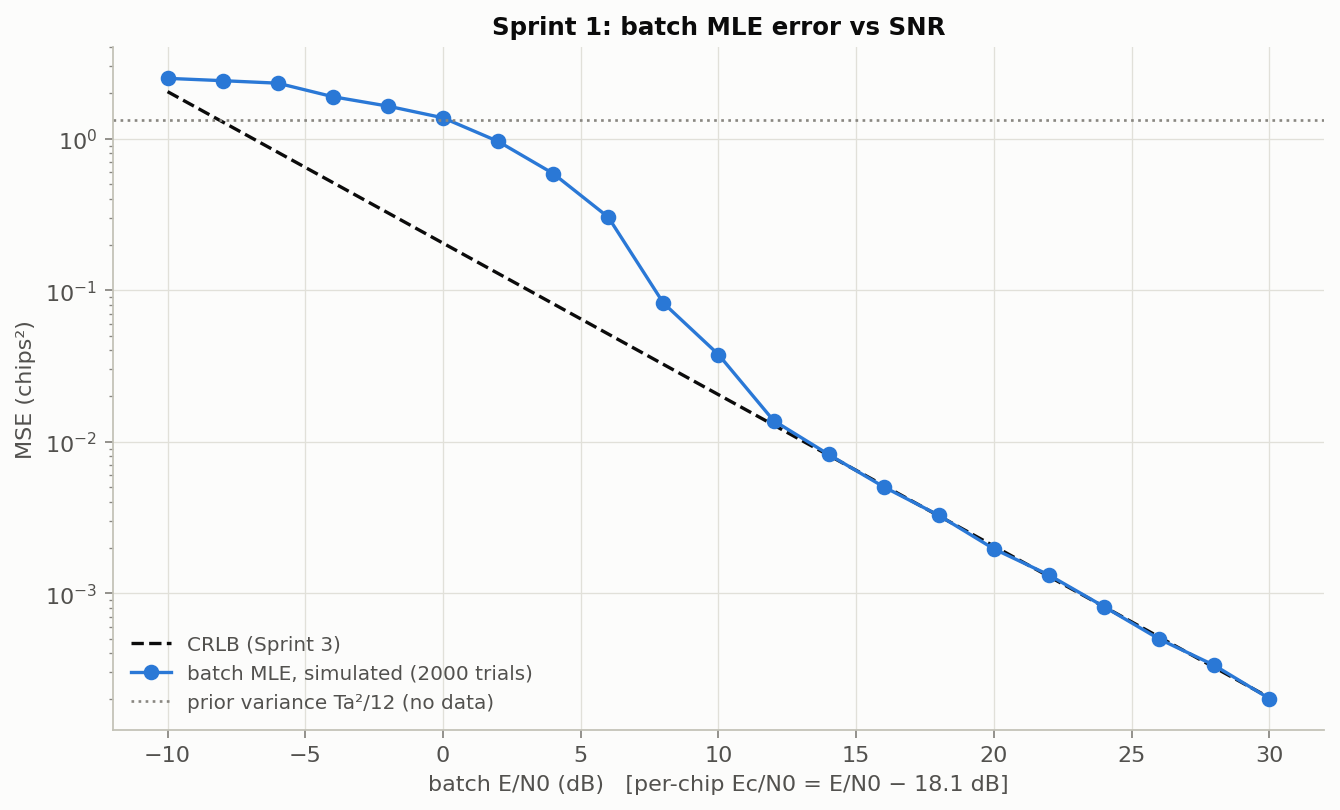
\includegraphics[width=0.78\textwidth]{s1_mle_mse_vs_snr.png}
\caption{Batch MLE MSE (2000 trials/point), CRLB and prior variance.}
\end{figure}
\begin{center}
\begin{tabularx}{\textwidth}{>{\raggedright\arraybackslash}p{3.4cm}>{\raggedright\arraybackslash}X>{\raggedright\arraybackslash}p{4.4cm}}
\toprule
\textbf{Regime} & \textbf{Evidence} & \textbf{Meaning}\\
\midrule
High SNR ($\ge$12--14\,dB) & MSE/CRLB $=0.997$ averaged over 14--30\,dB (points 0.96--1.03) & the MLE is efficient\\
Threshold ($\approx$6--12\,dB) & gross errors 0.8\% at 10\,dB, 2.1\% at 8\,dB, 8.7\% at 6\,dB & wrong-peak errors take over\\
Low SNR ($\le$0\,dB) & MSE above the prior variance; 3.09\,chips$^2$ on pure noise & no information; edge pile-up\\
\bottomrule
\end{tabularx}
\end{center}

\subsection{Sprint 2 --- the DLL works, with a limited pull-in range}
S-curve slope at zero 1.000; pull-in $\pm1.80$ chips; noise-free final error $\approx10^{-7}$ chips; locked MSE 1.04--1.09$\times$
CRLB (by design of $K$); some runs lose lock at 0\,dB.

\subsection{Sprint 3 --- the CRLB}
Implementation agrees with a frequency-domain computation to 0.05\%; the MLE attains it above threshold; three identified
reasons it fails below (Section~\ref{sec:crlb}); pilot dependence factor 2.4.

\subsection{Sprint 4 --- the ZZB is valid and informative}
Both limits reproduced (1.3323 vs 1.3333; 0.997$\times$CRLB at 40\,dB); the bound lies below the simulated MLE at every SNR within
the 95\% interval; it departs from the CRLB at 5.95\,dB.

\subsection{Sprint 5 --- four curves on one plot}
\begin{figure}[h]
\centering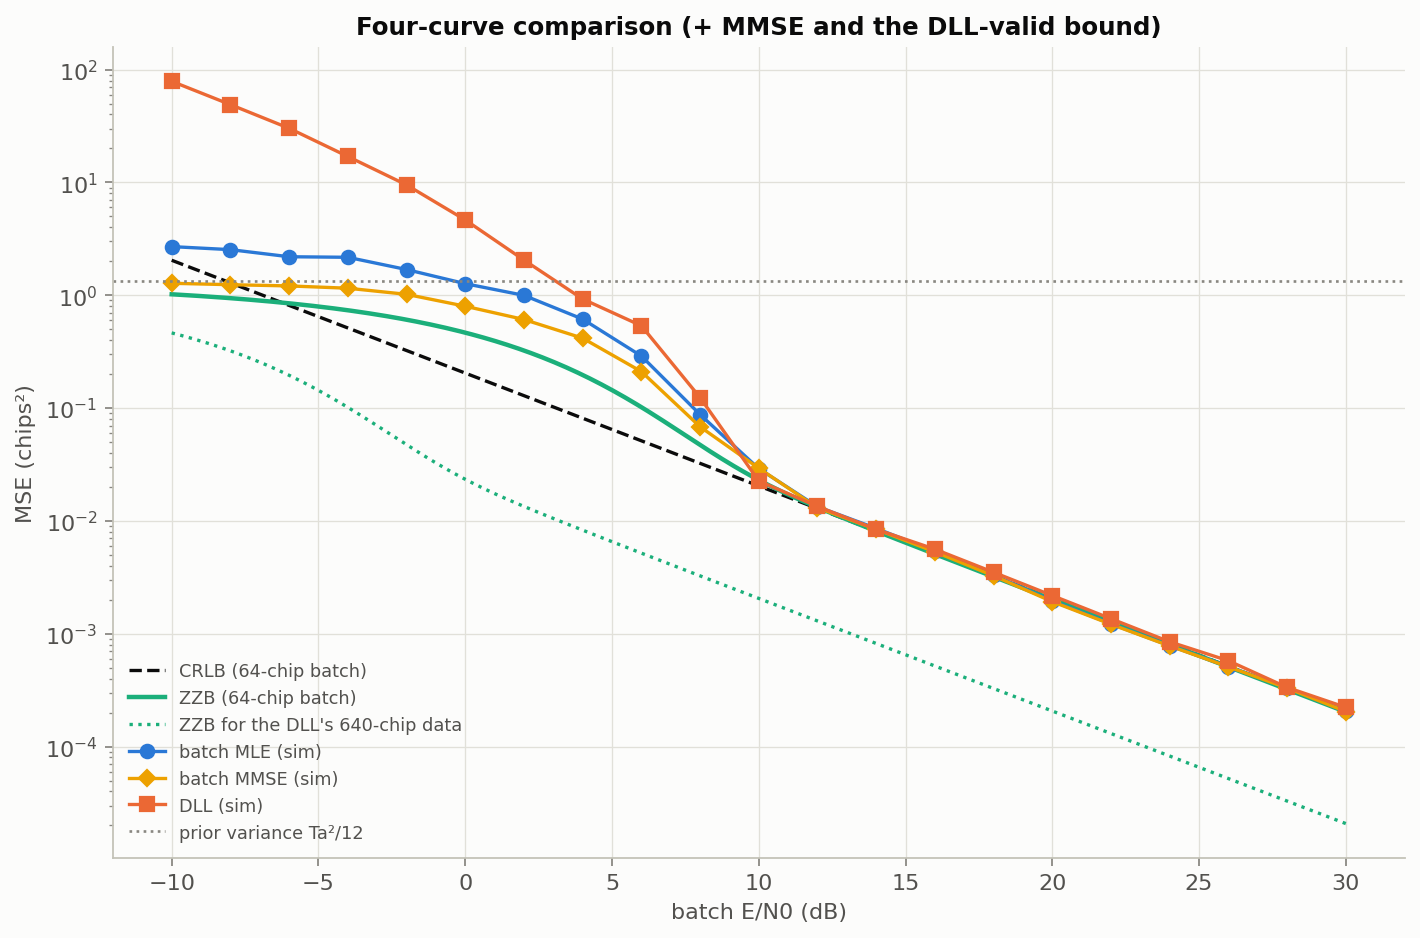
\includegraphics[width=0.82\textwidth]{s5_four_curves.png}
\caption{CRLB, ZZB, batch MLE, batch MMSE and DLL, plus the ZZB for the DLL's own 640-chip data (dotted) --- the only bound
valid for the DLL.}
\end{figure}
\begin{itemize}
\item Above $\approx$12\,dB everything sits on the 64-chip CRLB (DLL slightly above, by design).
\item At low SNR the MMSE levels off at the prior variance as the ZZB predicts ($-10$\,dB: MMSE 1.28, ZZB 1.02, MLE 2.70).
\item Below threshold the DLL is far worse than both batch estimators, and stays above the ZZB for its own data.
\end{itemize}
\begin{figure}[h]
\centering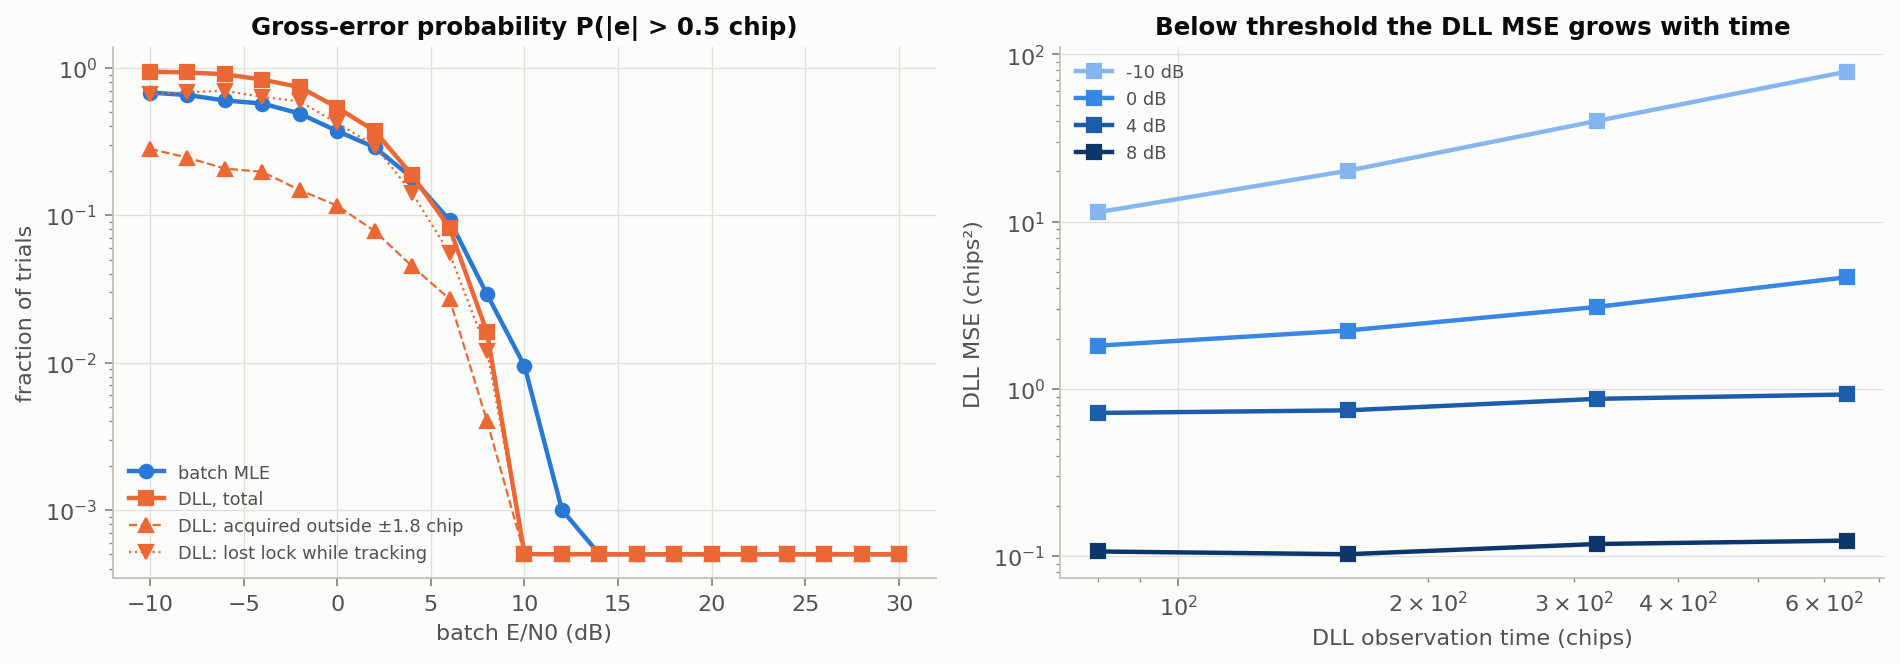
\includegraphics[width=\textwidth]{s6_dll_failure_mechanisms.png}
\caption{Left: gross-error probability; DLL failures split into acquisition outside the pull-in range and loss of lock (they
add up to the total). Right: below threshold the DLL's MSE grows with observation time.}
\end{figure}
At 0\,dB, 54\% of DLL runs end with a gross error: 12\% acquired outside the pull-in range, 42\% lost lock while tracking.

\subsection{Sprint 6 --- the threshold, located precisely}\label{sec:res6}
\begin{figure}[h]
\centering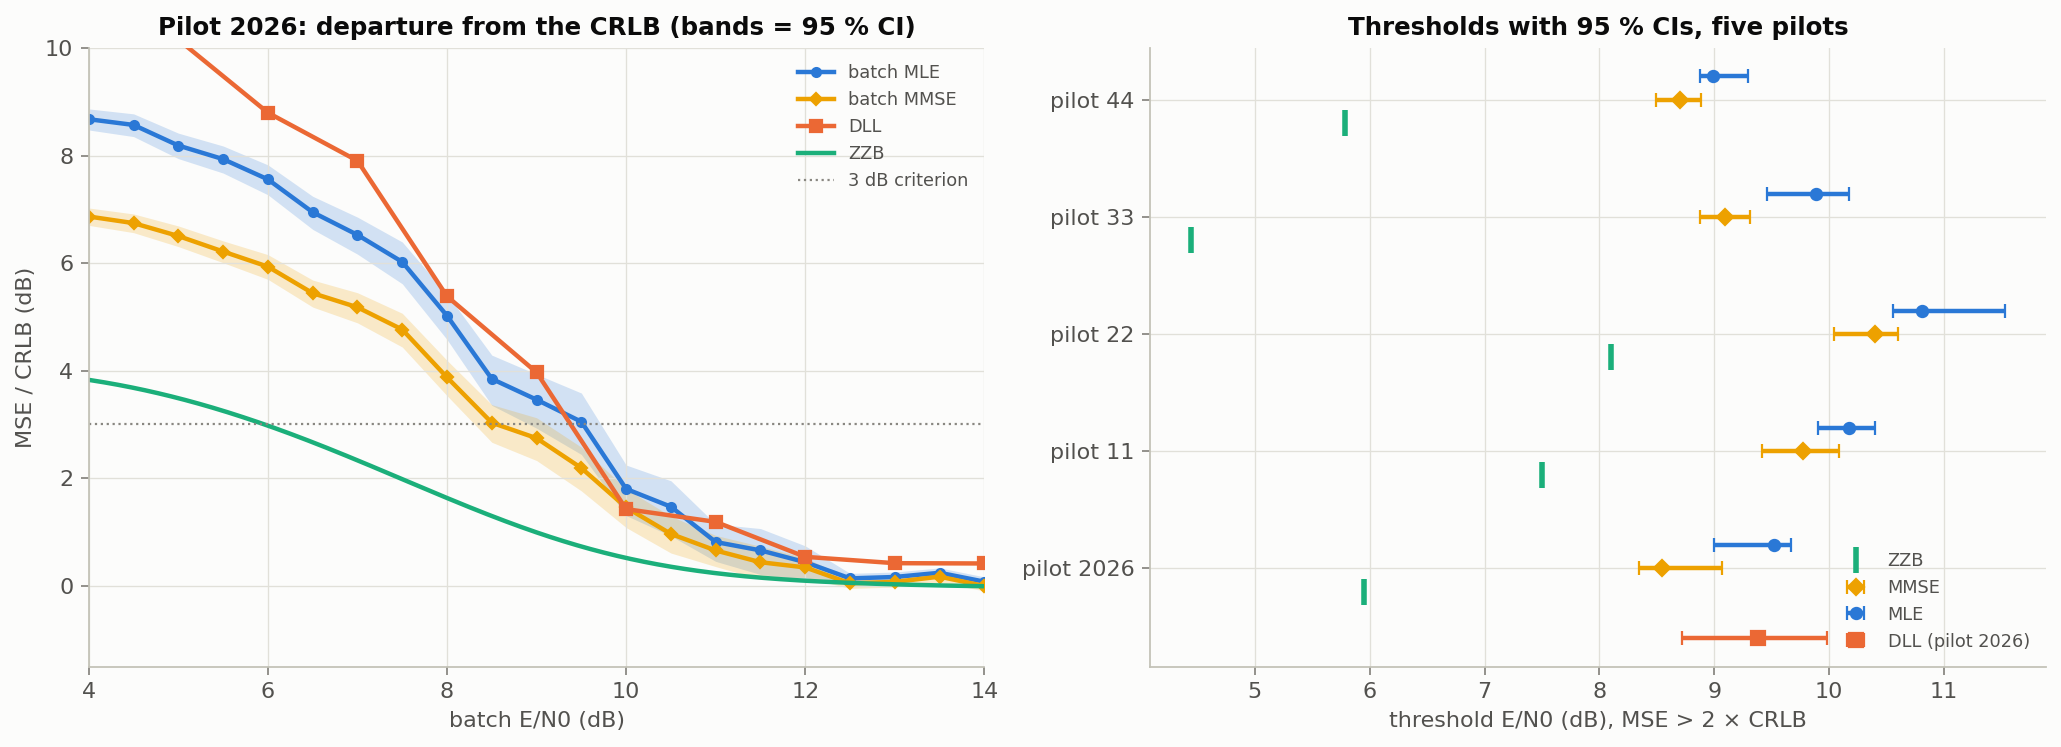
\includegraphics[width=\textwidth]{s6_threshold_precise.png}
\caption{Left: departure from the CRLB with 95\% bands (pilot 2026; 20{,}000 trials/point for MLE/MMSE, 4000 for the DLL). Right:
thresholds with 95\% CIs for five random pilots.}
\end{figure}
\begin{center}
\begin{tabular}{lcc}
\toprule
\textbf{Pilot 2026, MSE criterion} & \textbf{Threshold} & \textbf{95\% CI}\\
\midrule
ZZB (bound) & 5.95\,dB & ---\\
Batch MMSE (best possible estimator) & 8.54\,dB & [8.35, 9.07]\\
Batch MLE & 9.52\,dB & [9.00, 9.66]\\
DLL & 9.38\,dB & [8.72, 9.98]\\
\bottomrule
\end{tabular}
\end{center}
\textbf{The gap to the bound splits in two:} bound looseness MMSE$-$ZZB $=2.59$\,dB and MLE sub-optimality MLE$-$MMSE $=0.85$\,dB
(CI 0.25--1.24, significant). About three-quarters of the gap is the bound being optimistic --- built from \emph{pairwise} tests
while an estimator must reject \emph{all} competing delays.

\textbf{Five pilots:} MLE$-$ZZB ranges 2.7--5.4\,dB (mean 3.5); MMSE$-$ZZB 2.3--4.7\,dB (mean 2.9); the MMSE leads the MLE for every
pilot. The ZZB threshold moves a lot (4.4--8.1\,dB) and nearly follows $\beta^2$, while the MLE threshold moves less (9.0--10.8\,dB):
thresholds are defined relative to each pilot's own CRLB.

\textbf{DLL vs MLE depends on the criterion:}
\begin{itemize}
\item MSE criterion: DLL$-$MLE $=-0.12$\,dB, CI $[-0.87,0.59]$ --- \textbf{not significant}.
\item Gross-error criterion: DLL 8.81\,dB vs MLE 9.49\,dB --- the DLL is \textbf{0.68\,dB more robust} (CI 0.40--0.99): it observes
640 chips and recovers from wrong acquisitions within its pull-in range.
\item Far below threshold the DLL is much worse (loss of lock, unbounded drift).
\end{itemize}
\textbf{Subtlety:} the MMSE has a lower MSE threshold but a slightly higher gross-error threshold than the MLE (9.63 vs 9.49\,dB):
by hedging between peaks it makes more moderate errors just above 0.5 chip and fewer very large ones.

\subsection{Supplement --- the prior width moves the threshold}
\begin{figure}[h]
\centering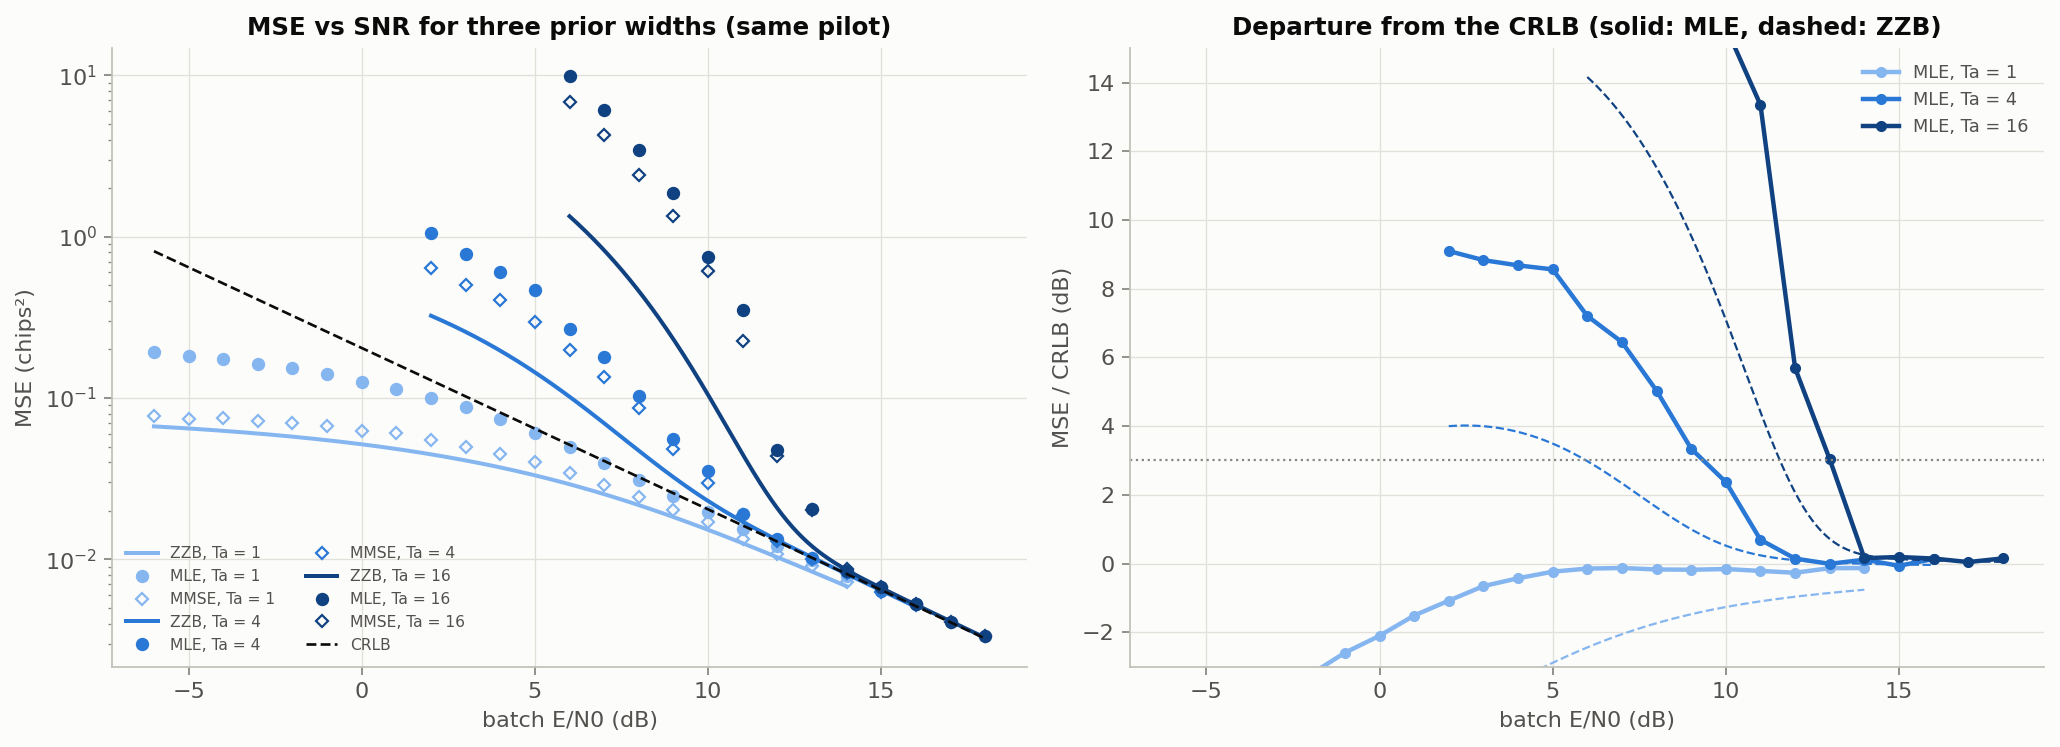
\includegraphics[width=\textwidth]{s6_prior_width.png}
\caption{Same pilot, prior widths 1, 4 and 16 chips (10{,}000 trials/point).}
\end{figure}
\begin{center}
\begin{tabular}{ccccc}
\toprule
$T_a$ & ZZB & MMSE (95\% CI) & MLE (95\% CI) & MLE$-$ZZB\\
\midrule
1 chip & none & masked & masked & ---\\
4 chips & 5.95\,dB & 8.84 [8.58, 9.14] & 9.34 [8.81, 10.08] & 3.4\,dB\\
16 chips & 11.56\,dB & 12.99 [11.97, 13.37] & 13.01 [11.95, 13.41] & 1.5\,dB\\
\bottomrule
\end{tabular}
\end{center}
A wider window has more places for a winning noise peak, so the threshold moves up $\approx3.7$\,dB from $T_a=4$ to 16. With
$T_a=1$ there is no distant peak: the threshold is \textbf{masked}. The ZZB is relatively tighter for the wide prior (gap
$3.4\to1.5$\,dB) --- observed, not yet explained.

% =====================================================================
\section{Decision log and the mistakes we fixed}\label{sec:decisions}
\begin{center}
\begin{tabularx}{\textwidth}{>{\raggedright\arraybackslash}p{1.6cm}>{\raggedright\arraybackslash}X>{\raggedright\arraybackslash}X}
\toprule
\textbf{When} & \textbf{Decision / correction} & \textbf{Why}\\
\midrule
Sprint 1 & m-sequence script replaced by the raised-cosine, random-delay model & ZZB needs a prior; exact delay; analytic spectrum\\
Oct 6 & prior width 1 $\to$ 4 chips & with 1 chip the threshold is masked\\
Oct 6 & DLL given the MLE's pilot, repeated & a different pilot made the DLL appear to beat the CRLB\\
Oct 6 & block replicas, offset calibration, constant gain & removed biases of 33\% and 100\% of the CRLB and a noise blow-up\\
Oct 7 & error bars and two threshold criteria & 2000 trials on a 2-dB grid could not support ``DLL 1.2\,dB worse''\\
Oct 7 & pull-in corrected 0.75 $\to$ 1.8 chips; failure classes partition the total & measured S-curve; overlapping categories\\
Oct 7 & ``DLL $\approx$ CRLB is a bound'' withdrawn & the match is by design of $K$\\
Oct 7 & ZZB for the DLL's own data added & only valid bound for the DLL\\
Oct 7 & DLL windows follow its own timing & fixed windows distorted low-SNR behaviour\\
Oct 9 & pulse tapered over its last chip & hard cut made the ZZB miss the CRLB limit by $\sim$1\%\\
Oct 9--12 & conditional bias instead of averaged bias; ``gap mostly MLE sub-optimality'' corrected & averaged bias cancels; MMSE only $\approx$0.85\,dB better\\
Nov 5 & ``DLL not different from MLE'' refined & true for MSE, false for gross errors\\
Nov 5 & novelty claim narrowed & batch ZZB for GNSS code tracking already exists\\
\bottomrule
\end{tabularx}
\end{center}

% =====================================================================
\section{What the four surveys taught us}\label{sec:surveys}
\begin{center}
\begin{tabularx}{\textwidth}{>{\raggedright\arraybackslash}p{3.4cm}>{\raggedright\arraybackslash}p{4.0cm}>{\raggedright\arraybackslash}X}
\toprule
\textbf{Survey} & \textbf{Method} & \textbf{Lesson}\\
\midrule
01 Independent validation (Oct 7) & literature check, re-implementation, adversarial audit & theory and code correct; several \emph{claims} wrong $\to$ fixes and error bars\\
02 Literature survey (Oct 13) & annotated bibliography, gap searches & everything up to the batch threshold is a reproduction\\
03 Deep-research check (Oct 13) & multi-agent search, 25 claims $\times$ 3 verifiers & optimal-MTLL theory exists for \emph{phase}; claim must be about code delay and the bound--MTLL link\\
04 Interdisciplinary \& second novelty check (Nov 5) & targeted searches & batch ZZB for GNSS code tracking exists (Emmanuele 2012, Liu 2016); natural bridge = state estimation and integrity; robotics/VLM links would be forced\\
\bottomrule
\end{tabularx}
\end{center}
\begin{resultbox}[Cumulative position]
\textbf{Reproduction:} MLE, CRLB, ZZB for delay, MLE threshold prediction, batch ZZB for GNSS code tracking, linear DLL theory,
DLL MTLL. \textbf{Our own observations:} ZZB looseness against the MMSE (2.6 + 0.85\,dB), its pilot dependence and prior-width
trend, the DLL failure decomposition, the criterion-dependent DLL-vs-MLE comparison. \textbf{Appears open (medium-low
confidence):} bounds with tracking dynamics linked to loss of lock, for PN code delay. \textbf{Rule:} always ``we found no prior
work that\ldots'', never ``first''.
\end{resultbox}

% =====================================================================
\section{Limitations}\label{sec:limits}
\begin{itemize}
\item Synthetic data only (needed for ground truth and bound comparison).
\item Constant delay (no Doppler); coherent tracking with known amplitude and phase.
\item Known pilot (no unknown data bits); no multipath.
\item One DLL design ($d=0.5$, 4-chip updates, one loop gain).
\item The batch ZZB is not a bound for the DLL; the 640-chip ZZB is valid but loose.
\item The pilot spread and the prior-width trend of the gap are measured but not explained.
\item Novelty of the proposed extension is uncertain (absence-of-evidence argument).
\end{itemize}

% =====================================================================
\part{The remaining 30\%}
\section{Proposal: where does a delay tracker lose information?}\label{sec:proposal}
\prop\ --- nothing in this section is implemented. Full text: \texttt{docs/evaluation/research\_proposal.md}.

\subsection{Directions considered}
\begin{center}
\begin{tabularx}{\textwidth}{>{\raggedright\arraybackslash}X>{\raggedright\arraybackslash}p{3.6cm}>{\raggedright\arraybackslash}p{2.0cm}>{\raggedright\arraybackslash}p{2.4cm}}
\toprule
\textbf{Direction} & \textbf{Novelty} & \textbf{Feasible} & \textbf{Verdict}\\
\midrule
D1 Dynamic decomposition of the tracking threshold (bound / estimator / loop) & medium & yes (core) & \textbf{recommended}\\
D2 Loss-of-lock risk prediction (integrity for autonomous navigation) & medium & yes & part of D1 (H4)\\
D3 Adaptive loop bandwidth via control / RL & low (adaptive-bandwidth methods exist) & partly & not pursued\\
D4 Pilot/code selection by threshold & low--medium (ZZB waveform design exists) & yes & side project\\
D5 Robot localisation with UWB ranging & low; physics mismatch (NLOS, not thermal threshold) & risky & forced --- not pursued\\
\bottomrule
\end{tabularx}
\end{center}

\subsection{Research question and intuition}
Our static study split the gap to the bound into \emph{bound looseness} (ZZB$\to$MMSE, 2.6\,dB) and \emph{estimator sub-optimality}
(MMSE$\to$MLE, 0.85\,dB). Tracking adds \textbf{memory} (each step's prior is the previous posterior, narrowing the search window)
and \textbf{feedback} (the DLL commits to one estimate and can be pushed outside its pull-in range --- loss of lock).
\textbf{Question:} for a moving delay, how much of a DLL's low-SNR failure is fundamental, how much is sub-optimal estimation,
and how much is loss of lock --- and can loss of lock be predicted quantitatively?

\subsection{Model}
\begin{equation}
d_k=d_{k-1}+w_k,\quad w_k\sim\mathcal N(0,q);\qquad r_k[n]=s_k(t_n-d_k)+v_k[n],\quad v_k[n]\sim\mathcal N(0,\sigma^2),
\end{equation}
one update $k$ per block of $M$ chips, with $\ln p(\br_k\mid d)=J_k(d)/\sigma^2+\text{const}$ (Section~\ref{sec:mle}).

\subsection{The optimal tracker --- an exact grid Bayes filter}
\begin{equation}
p(d_k\mid\br_{1:k})\ \propto\ \underbrace{e^{J_k(d_k)/\sigma^2}}_{\text{update}}\ \underbrace{\int\mathcal N(d_k;d_{k-1},q)\,p(d_{k-1}\mid\br_{1:k-1})\,dd_{k-1}}_{\text{prediction (Gaussian convolution)}}.
\end{equation}
The state is one-dimensional, so the recursion can be computed essentially exactly on a fine grid (point-mass filter, Bucy
\& Senne 1971); its posterior mean is the MMSE tracker, free of Monte Carlo approximation error.

\subsection{The posterior CRB for this model --- derivation}
Tichavský, Muravchik \& Nehorai (1998): $J_k=D_{22}-D_{21}(J_{k-1}+D_{11})^{-1}D_{12}$ with
$D_{11}=\E[-\partial^2_{d_{k-1}}\ln p(d_k\mid d_{k-1})]=1/q$, $D_{12}=D_{21}=-1/q$, $D_{22}=1/q+J_D$, where $J_D=\sum_ns_k'(t_n)^2/\sigma^2$
(Section~\ref{sec:crlb}). Substituting,
\begin{equation}
J_k=\frac1q+J_D-\frac{1/q^2}{J_{k-1}+1/q}=J_D+\frac{J_{k-1}}{q\,J_{k-1}+1}=J_D+\frac{1}{q+1/J_{k-1}}.
\end{equation}
With $R=1/J_D$ and $P=1/J$, the fixed point satisfies $P^2+qP-qR=0$:
\begin{equation}
P_\infty=\tfrac12\Big(-q+\sqrt{q^2+4qR}\Big),\qquad K_\infty=\frac{P_\infty+q}{P_\infty+q+R},
\end{equation}
the steady-state scalar Kalman filter.
\begin{proofbox}[Check of the fixed point]
Kalman: prediction $P^-=P+q$, update $P=P^-R/(P^-+R)$. At steady state $P(P+q+R)=(P+q)R\Rightarrow P^2+qP-qR=0$.\hfill$\blacksquare$
\end{proofbox}
\textbf{Link to our DLL:} $\theta_{k+1}=\theta_k-KD_k$ with $D_k\approx\varepsilon_k+n_k$ is a fixed-gain Kalman filter in the linear
regime; $K=K_\infty$ makes it optimal there --- replacing our Sprint-2 gain rule with a principled one.

\subsection{Loss of lock as a Markov chain}
With the measured S-curve $D(\varepsilon)$ and discriminator noise of variance $\sigma_D^2$,
$\varepsilon_{k+1}=\varepsilon_k-K\,D(\varepsilon_k)-K\,n_k+w_{k+1}$ is a one-dimensional Markov chain. Discretise $\varepsilon$ inside the
lock region $|\varepsilon|<R_{\rm pull}\approx1.8$ chips; the mean exit times satisfy the first-step equations
\begin{equation}
m(\varepsilon)=1+\sum_{\varepsilon'}P(\varepsilon\to\varepsilon')\,m(\varepsilon'),\qquad m=0\text{ outside the lock region},
\end{equation}
i.e.\ one linear solve $(I-P_{\rm in})\mathbf m=\mathbf 1$; the mean time to lose lock is $m(0)$. Published MTLL results are
mostly continuous-time, second-order loops at small-noise asymptotics; this discrete first-order version uses our measured
S-curve and can be checked against simulation.

\subsection{Risk score (applied part)}
From the optimal tracker's posterior:
$\rho_k=P\big(|d_k-\hat\theta^{\rm DLL}_k|>R_{\rm pull}\mid\br_{1:k}\big)$, compared with a classical correlator-power lock
detector by ROC curve and detection lead time --- relevant to integrity monitoring in autonomous navigation.

\subsection{Hypotheses --- each can fail}
\begin{center}
\begin{tabularx}{\textwidth}{l>{\raggedright\arraybackslash}X>{\raggedright\arraybackslash}p{3.0cm}>{\raggedright\arraybackslash}p{3.6cm}}
\toprule
 & \textbf{Hypothesis} & \textbf{Test} & \textbf{If it fails}\\
\midrule
H1 & Above threshold, DLL($K_\infty$) and the grid tracker both attain the PCRB & RMSE vs $E_c/N_0$ & diagnose implementation or nonlinear jitter\\
H2 & The DLL leaves the PCRB earlier; conditioning on lock removes most of the excess & lock-conditioned RMSE & excess is jitter inside lock --- quantify via the chain\\
H3 & Markov-chain MTLL matches simulation; DLL threshold where MTLL $\approx$ horizon & MTLL vs $E_c/N_0$, $K$ & refine the discretisation\\
H4 & The posterior risk score predicts loss of lock earlier than a classical detector & ROC/AUC, lead time & report where each wins\\
\bottomrule
\end{tabularx}
\end{center}

\subsection{Experiments and roadmap}
\textbf{E1} RMSE vs $E_c/N_0$ (PCRB, grid tracker, linearised Kalman, DLL($K_\infty$), 2--3 values of $q$, bootstrap CIs);
\textbf{E2} lock-conditioned DLL RMSE; \textbf{E3} Markov-chain vs simulated MTLL; \textbf{E4} risk score vs correlator-power detector;
\textbf{ablations} early--late spacing, five pilots; \textbf{stretch} a sequential ZZB or the marginal WWB (Fritsche et al.\ 2015).
\begin{center}
\begin{tabularx}{\textwidth}{l>{\raggedright\arraybackslash}X>{\raggedright\arraybackslash}p{3.6cm}l}
\toprule
\textbf{Week} & \textbf{Work} & \textbf{Deliverable} & \textbf{Priority}\\
\midrule
1 & random-walk model, PCRB, grid tracker, DLL($K_\infty$), E1; tests & notebook 08 & P0\\
2 & E2, Markov-chain MTLL (E3) & notebook 09 & P0\\
2 & risk score (E4), ablations & figures, table & P1\\
3 & stretch bound; report and final presentation & report, slides & P0 / P2\\
\bottomrule
\end{tabularx}
\end{center}

\subsection{How it differs from existing work}
\begin{center}
\begin{tabularx}{\textwidth}{>{\raggedright\arraybackslash}p{4.6cm}>{\raggedright\arraybackslash}X>{\raggedright\arraybackslash}X}
\toprule
\textbf{Existing} & \textbf{What it does} & \textbf{What D1 adds}\\
\midrule
Emmanuele et al.\ 2012; Liu et al.\ 2016 & ZZB for one integration period of GNSS signals & tracking dynamics; decomposition bound / estimator / loop\\
Holmes \& Biederman 1978; Hasson \& Bobrovsky 1995; Groh et al.\ 2012 & MTLL of given loops & link MTLL to the MSE threshold and the optimal tracker\\
Tichavský 1998; Rapoport \& Oshman 2007; Fritsche 2015 & generic recursive bounds & applied to PN code tracking against an exact optimal tracker\\
Fischler \& Schuss 2007 & optimal-MTLL filtering for phase & code delay (non-periodic, code-dependent side-lobes)\\
\bottomrule
\end{tabularx}
\end{center}

% =====================================================================
\part{Rehearsal}
\section{Question bank with follow-ups}\label{sec:qa}
\newcommand{\Q}[1]{\par\medskip\noindent\textbf{#1}\par}
\newcommand{\A}[1]{\noindent\hangindent=1.5em\hangafter=0 #1\par}
\newcommand{\F}[1]{\noindent\hangindent=1.5em\hangafter=0 \textcolor{black!65}{\textit{Follow-up:} #1}\par}

\subsection*{A. Concepts}
\Q{A1. What is your project in one sentence?}
\A{We estimate the delay of a known BPSK signal with a batch MLE and a DLL and compare them with the CRLB and the ZZB, to understand the low-SNR threshold where errors suddenly become large.}
\Q{A2. What exactly is the threshold effect?}
\A{A change in the type of error: above threshold the estimate sits on the true correlation peak; below it, noise sometimes makes a wrong peak win and the estimate jumps chips away.}
\F{Is it a sharp transition? --- No, a region a few dB wide; hence fixed criteria and confidence intervals.}
\Q{A3. Why plot MSE rather than variance?}
\A{Below threshold the estimators are biased for a given delay, and the ZZB bounds MSE; MSE = variance + bias$^2$.}
\Q{A4. Why is the CRLB not valid at low SNR?}
\A{It assumes unbiasedness, it is local, and it ignores the prior --- below $-8$\,dB it exceeds the prior variance.}
\F{So is the CRLB wrong? --- No; it bounds a class of estimators ours leave at low SNR. It is not informative there.}
\Q{A5. Can an estimator beat the CRLB?}
\A{Yes: a biased one; a constrained one near the window edge (MSE/CRLB $=0.63$ there); one using more data than the CRLB assumes.}
\Q{A6. Why does the ZZB need a prior? Is a uniform prior realistic?}
\A{It bounds the MSE averaged over the prior, which keeps it finite at zero SNR. Uniform models ``somewhere in this window'' after coarse acquisition.}
\F{Dependence on $T_a$? --- $T_a=1$: threshold masked; $4\to16$: threshold rises $\approx3.7$\,dB and the ZZB gap shrinks $3.4\to1.5$\,dB.}

\subsection*{B. Model and implementation}
\Q{B1. Why a raised-cosine pulse?}
\A{CRLB $=1/(2(\ENo)\beta^2)$; rectangular chips have $\beta^2=\infty$, so the CRLB would be 0. Real receivers band-limit.}
\Q{B2. Why 4 samples per chip?}
\A{The spectrum ends at 0.75 cycles/chip, below Nyquist (2): samples hold all information and sums equal integrals.}
\Q{B3. Why did you taper the pulse?}
\A{A hard cut left a small slope jump that broke $\rho''(0)=-\beta^2$, so the ZZB missed the CRLB limit by $\sim$1\%. The taper only touches $5<|t|\le6$.}
\Q{B4. Why does the MLE need no SNR but the MMSE does?}
\A{$\sigma^2$ scales the whole log-likelihood (arg-max unchanged); the posterior mean weights by $e^{J/\sigma^2}$.}
\Q{B5. Why did the model change after the first Sprint-1 script?}
\A{The ZZB needs a random delay with a prior; exact analytic delay; analytic spectrum. Same qualitative result.}

\subsection*{C. Derivations (expect the board)}
\Q{C1. Derive the MLE.}
\A{Gaussian likelihood, expand the square, drop $\sum r^2$, maximise $J(\theta)$ (Section~\ref{sec:mle}).}
\Q{C2. Derive the CRLB, including the inequality.}
\A{$\E[(\hat\theta-\theta)S]=1$ and Cauchy--Schwarz (Section~\ref{sec:crlbthm}); then $I=\frac1{\sigma^2}\sum s'^2$ (Section~\ref{sec:crlb}).}
\F{Why is $\beta^2$ the Gabor bandwidth? --- Parseval: differentiation multiplies the spectrum by $j2\pi f$.}
\Q{C3. Prove $\E[X^2]=\int_0^\infty2xP(X\ge x)dx$.}
\A{$X^2=\int_0^\infty2x\mathbf 1\{X\ge x\}dx$; take expectations and swap (Tonelli).}
\Q{C4. Why is any estimator's tail probability bounded by $P_{\min}$?}
\A{Use it as a detector (decide $H_1$ iff $\hat\tau\ge\varphi+h/2$); its errors are exactly the tail events; no detector beats the optimal one.}
\Q{C5. Why is $P_{\min}=Q(\sqrt{(\ENo)(1-\rho(h))})$?}
\A{Equal priors, known signals in white noise: $Q(\|\bs_1-\bs_0\|/2\sigma)$ with $\|\bs_1-\bs_0\|^2=2\sum s^2(1-\rho)$.}
\Q{C6. Show ZZB $\to$ CRLB at high SNR.}
\A{$1-\rho\approx\frac12\beta^2h^2$; $\int_0^\infty hQ(ah)dh=1/(4a^2)$ by parts; $a^2=\frac12(\ENo)\beta^2$.}
\F{Why $\rho''(0)=-\beta^2$? --- summation by parts: $\sum s\,s''=-\sum s'^2$.}
\Q{C7. Show ZZB $\to T_a^2/12$ with no signal.}
\A{$Q(0)=\frac12$ and $\int_0^{T_a}\frac h2(1-\frac h{T_a})dh=T_a^2/12$.}
\Q{C8. What is valley filling and does it matter?}
\A{Replacing the integrand by its non-increasing envelope (valid since the tail probability decreases in $h$); here $<0.01\%$.}
\Q{C9. Derive the DLL's noise averaging.}
\A{$\varepsilon_{j+1}=(1-K)\varepsilon_j-Kn_j$, impulse response $K(1-K)^k$, $\sum h_k^2=K/(2-K)$, so $N_{\rm eff}=(2-K)/K$.}
\Q{C10. Why is early minus late proportional to the error?}
\A{$R(\varepsilon-\frac d2)-R(\varepsilon+\frac d2)\approx-2R'(\frac d2)\varepsilon$.}

\subsection*{D. DLL vs MLE}
\Q{D1. Why $d=0.5$ chip?}
\A{Narrower spacing approximates the derivative better but shrinks the linear region; 0.5 is a standard compromise.}
\Q{D2. Where does $K=2/17$ come from?}
\A{$N_{\rm eff}=16$ updates = 64 chips, the batch length: $K=2/(N_{\rm eff}+1)$.}
\F{So DLL $\approx$ CRLB is by construction? --- Yes; a narrower loop goes below the 64-chip CRLB because it uses more data.}
\Q{D3. Is the comparison fair?}
\A{In steady state yes; near threshold no --- the DLL sees 640 chips. Hence the ZZB for the DLL's own data, the only bound valid for it.}
\Q{D4. Isn't the offset calibration cheating?}
\A{It uses only the known pilot; with deliberately wrong timing the results were identical. Without it the DLL is biased.}
\Q{D5. Which is better, DLL or MLE?}
\A{Equal above threshold (by design); near threshold the same MSE threshold but fewer gross errors for the DLL (0.68\,dB); far below threshold the DLL is much worse (loss of lock).}
\Q{D6. Why a first-order loop?}
\A{Constant delay, no Doppler: no steady-state error. With Doppler a second-order loop is needed.}

\subsection*{E. Experiments}
\Q{E1. How reliable are your numbers?}
\A{Up to 20{,}000 trials per point, bootstrap CIs, fixed seeds, tests against analytic facts, independent re-implementation and audit.}
\Q{E2. The 3\,dB threshold definition looks arbitrary.}
\A{Fixed before running; a second, outlier-robust definition is also reported; we say when they differ.}
\Q{E3. The ZZB is 3.6\,dB below your MLE threshold. Is the ZZB wrong?}
\A{Both limits match and an independent implementation agrees to 0.12\%. The gap = 2.6\,dB bound looseness + 0.85\,dB MLE sub-optimality; it depends on the pilot and shrinks for a wider prior.}
\F{Mallat et al.\ found their bound much tighter. --- Different signal (single pulse vs PN code) and definitions; no contradiction claimed.}
\Q{E4. Why does the MLE's MSE exceed the prior variance at very low SNR?}
\A{The arg-max of a noise process piles up at the window edges: 3.09 vs 1.33\,chips$^2$. The MMSE goes to 1.33.}
\Q{E5. Why synthetic data only?}
\A{The bounds need the exact model and ground truth; real data add Doppler, multipath, bits and clock effects.}

\subsection*{F. Novelty (answer honestly)}
\Q{F1. What is your own contribution?}
\A{The theory up to 70\% is known. Ours: a carefully verified study for one model plus observations not found stated for PN pilots (gap decomposition, pilot and prior-width dependence, DLL failure decomposition). The research contribution is the proposal.}
\Q{F2. Hasn't the ZZB been applied to GNSS code tracking?}
\A{Yes --- Emmanuele et al.\ (ICASSP 2012), Liu et al.\ (ION ITM 2016), for one integration period. We propose dynamics and loss of lock.}
\Q{F3. Isn't loss of lock solved by MTLL theory?}
\A{MTLL gives exit times of a given loop; we found no work linking it to an MSE bound or the optimal tracker's threshold.}
\Q{F4. How sure are you that it is novel?}
\A{Not sure --- medium-low. Our first survey missed the Emmanuele papers, which is why we say ``we found no prior work that\ldots''.}
\Q{F5. Why not deep learning or RL?}
\A{Nothing requires it: the optimal tracker is computable exactly on a 1-D grid.}

\subsection*{G. Future work}
\Q{G1. What if H2 fails?}
\A{Then the near-threshold loss is partly jitter inside lock --- itself measurable with the Markov chain.}
\Q{G2. Why a grid filter, not a particle filter?}
\A{One-dimensional state: a fine grid computes the Bayes recursion essentially exactly.}
\Q{G3. Link to robotics / autonomous systems?}
\A{The DLL is a feedback estimator and the optimal tracker is the Bayes filter used in robot localisation; predicting loss of lock is an integrity problem. Robot UWB data were rejected: their outliers are NLOS, not thermal.}
\Q{G4. How would this extend to a real receiver?}
\A{Add Doppler (2-D state, second-order loop), carrier phase, data bits, multipath; the grid filter stays feasible in 2-D.}

% =====================================================================
\appendix
\section{Notation and equation sheet}
\begin{center}
\begin{tabular}{ll}
\toprule
\textbf{Symbol} & \textbf{Meaning}\\
\midrule
$\tau,\hat\tau,e=\hat\tau-\tau$ & true delay, estimate, error (chips)\\
$N_c=64$, $f_s=4$ & pilot length (chips), samples per chip\\
$\alpha=0.5$ & raised-cosine roll-off\\
$\beta^2$ & mean-square (Gabor) bandwidth, 1/chip$^2$\\
$\ENo$, $E_c/N_0$ & batch / per-chip energy-to-noise ratio\\
$T_a$ & prior width (chips)\\
$\rho(h)$ & normalised autocorrelation\\
$d,K,B_L,N_{\rm eff}$ & early--late spacing, loop gain, noise bandwidth, effective averaging length\\
\bottomrule
\end{tabular}

\medskip
\begin{tabular}{ll}
\toprule
\textbf{Quantity} & \textbf{Formula}\\
\midrule
SNR & $\ENo=\sum s^2/(2\sigma^2)$\\
MLE & $\arg\max_\theta\sum r\,s(t-\theta)-\frac12\sum s(t-\theta)^2$\\
CRLB & $1/(2(\ENo)\beta^2)$, $\beta^2=\sum s'^2/\sum s^2$\\
ZZB & $\int_0^{T_a}h\,\VF\{(1-\frac h{T_a})Q(\sqrt{(\ENo)(1-\rho(h))})\}dh$\\
ZZB limits & $T_a^2/12$ (no signal); CRLB (strong signal)\\
DLL & $\theta_{j+1}=\theta_j-K(E-L-b_j)/\bar k$; $N_{\rm eff}=(2-K)/K$; $B_LT=K/(2(2-K))$\\
PCRB (proposal) & $J_k=J_D+1/(q+1/J_{k-1})$; $P_\infty=\frac12(-q+\sqrt{q^2+4qR})$\\
\bottomrule
\end{tabular}
\end{center}

\section{Key references}
\begin{itemize}
\item S.\,M.\ Kay, \emph{Fundamentals of Statistical Signal Processing, Vol.\ I: Estimation Theory}, Prentice Hall, 1993.
\item J.\ Ziv and M.\ Zakai, ``Some lower bounds on signal parameter estimation,'' \emph{IEEE Trans.\ Inf.\ Theory}, 15(3), 1969.
\item D.\ Chazan, M.\ Zakai and J.\ Ziv, ``Improved lower bounds on signal parameter estimation,'' \emph{IEEE Trans.\ Inf.\ Theory}, 21(1), 1975.
\item K.\,L.\ Bell, Y.\ Steinberg, Y.\ Ephraim and H.\,L.\ Van Trees, ``Extended Ziv--Zakai lower bound for vector parameter estimation,'' \emph{IEEE Trans.\ Inf.\ Theory}, 43(2), 1997.
\item A.\ Mallat et al., ``Statistics of the MLE and approximate upper and lower bounds,'' Parts 1--2, arXiv:1405.4645, 1405.4647, 2014.
\item A.\ Emmanuele, M.\ Luise, F.\ Zanier and M.\ Crisci, ``Modified Ziv--Zakai bound for time-of-arrival estimation of GNSS signal-in-space,'' \emph{ICASSP}, 2012.
\item Liu et al., ``The Ziv--Zakai bound for time-of-arrival estimation of new generation GNSS signals,'' \emph{ION ITM}, 2016.
\item J.\,W.\ Betz and K.\,R.\ Kolodziejski, ``Generalized theory of code tracking with an early-late discriminator,'' Parts I--II, \emph{IEEE Trans.\ Aerosp.\ Electron.\ Syst.}, 45(4), 2009.
\item S.\,A.\ Stephens and J.\,B.\ Thomas, ``Controlled-root formulation for digital phase-locked loops,'' \emph{IEEE Trans.\ Aerosp.\ Electron.\ Syst.}, 31(1), 1995.
\item W.\,K.\ Holmes and L.\ Biederman, ``Delay-lock-loop mean time to lose lock,'' \emph{IEEE Trans.\ Commun.}, 26(11), 1978.
\item A.\ Hasson and B.\,Z.\ Bobrovsky, ``A comparison of the mean time to lose lock in coherent/noncoherent DLL's,'' 1995.
\item I.\ Groh, C.\ Gentner and J.\ Selva, ``Analytical computation of mean time to lose lock for Langevin delay-locked loops,'' \emph{IEEE Trans.\ Commun.}, 60(11), 2012.
\item P.\ Tichavský, C.\,H.\ Muravchik and A.\ Nehorai, ``Posterior Cramér--Rao bounds for discrete-time nonlinear filtering,'' \emph{IEEE Trans.\ Signal Process.}, 46(5), 1998.
\item I.\ Rapoport and Y.\ Oshman, ``Weiss--Weinstein lower bounds for Markovian systems. Part 1: Theory,'' \emph{IEEE Trans.\ Signal Process.}, 55(5), 2007.
\item C.\ Fritsche et al., ``Marginal Weiss--Weinstein bounds for discrete-time filtering,'' \emph{ICASSP}, 2015.
\item E.\ Fischler and Z.\ Schuss, ``Nonlinear filtering with optimal MTLL,'' arXiv:math/0703524, 2007.
\item R.\,S.\ Bucy and K.\,D.\ Senne, ``Digital synthesis of non-linear filters,'' \emph{Automatica}, 7(3), 1971.
\end{itemize}
Full annotated lists: \texttt{docs/surveys/}.

\end{document}
